% !TeX root = ../../thesis.tex
\chapter{Results and Discussion}

\section{Performance of EOM-CC2 Methods}
This section examines the performance of the EA-EOM-CC2 method for calculating electron affinities. Previous work has shown that EA-EOM-CC2 performs adequately for dipole-bound states (DBSs), whilst tending to overestimate vertical electron affinities (VEAs) for valence-bound states (VBSs) \cite{paran2024performance}. The following analysis focuses on three aspects: the basis set dependence for DBSs in section \ref{sec:results:basis}, the method's performance for VBSs using a test set of quinones in section \ref{sec:results:quinones}, and the efficacy of CC2 in generating Dyson orbitals through comparison of photodetachment cross-sections calculated with EOM-CC2, EOM-CCSD and HF in section \ref{sec:results:crosssection}.

\subsection{Basis Set Dependence of EA-EOM-CC2 in Dipole Bound Anions} \label{sec:results:basis}

The basis set dependence of EA-EOM-CC2 for dipole-bound radical anions was evaluated using a test set of 14 DBS of organic molecules taking as reference EA-EOM-CCSD \cite{paran2024performance}. The results as summarised in Table \ref{tab:basis}. The binding energies range from less than 1 meV for acetone to approximately 26 meV for nitrobenzene. The table also shows how the binding energy does not correlate strongly with the magnitude of the dipole moment for different species. For instance, phenylisocyanide, which has a slightly lower dipole moment than benzaldehyde, exhibits an electron affinity nearly twice as large.\\

The basis set cardinality was varied from DZ to QZ for EA-EOM-CC2 and from DZ to TZ for CCSD, while keeping additional diffuse functions fixed at 6s3p, \textit{vide infra}, for heavy atoms and 3s for hydrogens, referred to as (6s3p). For the EA-EOM-CC2 method, the influence of diffuse functions was further explored by fixing the cardinality to TZ and incrementally increasing the number of diffuse functions from 2s1p for heavy atoms and 1s for hydrogens, referred to as (2s1p), to 8s4p for heavy atoms and 4s for hydrogens, referred to as (8s4p). The exponents of the diffuse functions are detailed in the methods' section \ref{sec:methods:basis}. For comparison, the dipole strength, calculated at the HF level, and Koopmans' theorem (KT), which estimates the binding energy using the energy of the lowest unoccupied molecular orbital, are also included.\\

Starting with the simplest approximation, KT predicts that all anions with an EOM-EA-CCSD binding energy below 10 meV are unbound. However, even for more strongly bound cases, Koopmans' theorem significantly underestimates the binding energy, capturing only 20\% of the binding energy for nitrobenzene, for example.\\

No DBS is found when only the 2s1p diffuse function are added. At the 6s3p level the DBS energy is converged with respect to the extra diffuse functions added to the basis set, deviating by less than 1 meV from the value obtained with the 8s4p diffuse function. The errors are more pronounced for smaller molecules, such as acetaldehyde and acetone. This could be attributed to the inability of functions centred on a few atoms to adequately cover the spatial extent of the DBS orbital. This reasoning may also explain why the DBS of acetaldehyde is only predicted by RI-EA-EOM-CC2/aug-cc-pVTZ+8s4p, as it employs the most diffuse functions. At the RI-EA-EOM-CCSD/aug-cc-pVTZ+8s4p, the DBS of acetaldehyde is found to be 0.84 meV, compared to the 0.76 meV of CC2.\\

The binding energy increases with higher cardinality, as expected, due to the increased flexibility of the basis set. However, this effect is less significant than the addition of diffuse functions. For instance, the difference between RI-EA-EOM-CCSD/aug-cc-pVDZ+6s3p and RI-EA-EOM-CCSD/aug-cc-pVTZ+6s3p is less than 1 meV for most cases. Smaller molecules with lower-energy DBSs tend to be more challenging; for example, a TZ basis is required to predict the DBS of acetone. In general, and especially for larger systems, the inclusion of diffuse functions is more critical than the cardinality of the basis set for dipole-bound anions.\\

CC2/aug-cc-pVTZ+6s3p consistently overestimates the binding energies across all molecules when compared to CCSD/aug-cc-pVTZ+6s3p. The mean absolute error (MAE) is 2.8 meV, with deviations reaching up to 10 meV for nitrobenzene. For this reason, using a smaller cardinality results in a cancellation of errors for CC2.
The aug-cc-pVDZ+6s3p basis set, when employed with CC2, yields the lowest MAE of 2.3 meV compared to the reference results.

\begin{landscape}
\begin{table}[p]
  \centering
  \caption[EOM-EA DBA basis set dependence.]{ Electron affinity of dipole-bound radical anions computed using different augmented Dunning basis sets and EOM-EA RI-CC2 and EOM-EA RI-CCSD \cite{paran2024performance}. Koopman' theorem (KT), and dipole moment, \textmu, calculated at the HF/aug-cc-pVTZ+6s3p level, and mean absolute error (MAE) taking CCSD/aug-cc-pVTZ+6s3p as reference are also given. The values are in meV and Debye respectively.}
\label{tab:basis}
  \begin{tabular}{cccccccccccc}
    \toprule
    & & \multicolumn{6}{c}{RI-CC2} & \multicolumn{2}{c}{RI-CCSD} & & \\
    \cmidrule(lr){3-8} \cmidrule(lr){9-10} 
    & & \multicolumn{4}{c}{aug-cc-pVTZ} & pVDZ & pVQZ & pVDZ & pVTZ & & \\
    \multicolumn{2}{c}{Molecule} & 2s1p & 4s2p & 6s3p & 8s4p & 6s3p & 6s3p & 6s3p & 6s3p & KT & \textmu \\
    \hline
    Acetaldehyde & \ce{CH3CHO} & -156.7 & -27.8 & -3.2 & 0.8 & -4.6 & -3.2 & -4.6 & -3.1 & -0.4 & 3.29 \\
    Acetone & \ce{(CH3)2CO} & -114.9 & -16.8 & 1.3 & 3.3 & -0.3 & 0.9 & -0.5 & 0.9 & -5.1 & 3.46 \\
    Acetonitrile & \ce{CH3CN} & -61.2 & 12.6 & 19.9 & 20.1 & 18.2 & 20.3 & 17.1 & 18.4 & 4.2 & 4.29 \\
    Benzaldehyde & \ce{C6H5CHO} & -97.1 & -2.1 & 8.9 & 9.6 & 7.4 & 9.1 & 3.4 & 4.6 & -4.9 & 3.77 \\
    N,N-Dimethylformamide & \ce{(CH3)2NCHO} & -81.1 & 5.4 & 14.1 & 14.4 & 13.2 & 14.4 & 13.3 & 13.7 & 1.9 & 4.48 \\
    DMSO & \ce{(CH3)2SO} & -84.5 & 4.0 & 15.4 & 16.1 & 14.8 & 15.5 & 14.7 & 14.9 & 2.1 & 4.63 \\
    Formamide & \ce{CH3NO} & -92.2 & 1.1 & 16.2 & 17.2 & 15.1 & 17.0 & 15.1 & 15.9 & 3.4 & 4.28 \\
    Methylisocyanide & \ce{CH3NC} & -95.1 & -0.5 & 10.0 & 10.5 & 9.5 & 10.1 & 8.8 & 9.0 & -1.8 & 3.59 \\
    Nitrobenzene & \ce{C6H5NO2} & -63.6 & 30.6 & 34.8 & 34.8 & 32.5 & -- & 25.0 & 25.9 & 5.4 & 5.15 \\
    Nitromethane & \ce{CH3NO2} & -82.9 & 5.7 & 14.2 & 14.7 & 13.0 & 14.7 & 12.9 & 13.7 & 3.5 & 4.10 \\
    Nitrosobenzene & \ce{C6H5NO} & -125.0 & 1.0 & 11.4 & -- & 9.9 & -- & 5.1 & 6.0 & -4.1 & 3.73 \\
    Phenylisocyanide & \ce{C6H5NC} & -82.7 & 8.6 & 16.3 & 16.5 & 15.2 & 16.7 & 9.0 & 9.2 & -4.9 & 3.61 \\
    Pyridazine & \ce{C4H4N2} & -80.7 & 20.5 & 26.3 & 26.4 & 25.0 & 26.7 & 18.6 & 19.1 & 1.7 & 4.41 \\
    Vinylene carbonate & \ce{C3H2O3} & -82.5 & 20.9 & 27.2 & 27.4 & 26.4 & 27.7 & 25.1 & 25.5 & 10 & 5.05 \\
    \cmidrule(lr){2-11} 
    & MAE & 105.3 & 8.8 & 2.8 & 3.4 & 2.3 & 2.4 & 0.8 & 0.0 & 12.0 & \\
    \bottomrule
\end{tabular}
\end{table}
\end{landscape}

\subsection{Performance of EA-EOM-CC2 on Valence Bound Radical Anion States of Quinones} \label{sec:results:quinones}

\begin{table}[h!]
  \centering
  \caption[EA-EOM-CC2 benchmark for quinone VBS.]{EA-EOM-CC2 benchmark for quinone VBS. Reference values from literature\cite{schulz2018systematic} include experimental adiabatic EAs and verical EA CCSD(T) calculations using aug-cc-pVDZ basis set with LPNO-CCSD extrapolation to higher cardinal numbers. The RI-CC2 calculations employed three basis sets: aug-cc-pVTZ+6s3p (abbreviated as VTZ+) built as described in section \ref{sec:methods:basis}, standard aug-cc-pVTZ (VTZ), and aug-cc-pVDZ (VDZ).}
  \label{tab:Quinones}
  \centering
  \begin{tabular}{cccccccc}
  \toprule
   & & \multicolumn{2}{c}{Ref. \cite{schulz2018systematic}} & \multicolumn{4}{c}{RI-CC2}  \\
   \cmidrule(lr){3-4} \cmidrule(lr){5-8}
   & & & CCSD(T) & SCS & \multicolumn{3}{c}{No SCS} \\
  \cmidrule(lr){6-8}
  Molecule & \# & Exp. & +E\textsubscript{CBS} & VTZ+ & VTZ+ & VTZ & VDZ  \\
  \midrule
  Benzoq. & 1  & 1.91 & 1.64 & 1.54 & 2.02 & 2.02 & 1.81 \\
  Methylbenzoq. & 2  & 1.85 & 1.57 &  --  & 1.95 & 1.95 & 1.74 \\
  2,5-Dimethylbenzoq. & 3  & 1.76 & 1.49 & 1.39 & 1.89 & 1.89 & 1.68 \\
  2,6-Dimethylbenzoq. & 4  & 1.77 & 1.50 & 1.40 & 1.89 & 1.89 & 1.68 \\
  Trimethylbenzoq. & 5  & 1.69 & 1.43 & 1.34 & 1.84 & 1.84 & 1.63 \\
  Duroq. & 6  & 1.62 & 1.42 & 1.32 & 1.83 & 1.83 & 1.62 \\
  2,6-Dimethoxybenzoq. & 7  & 1.72 & 1.32 & 1.17 & 1.65 & 1.65 & 1.43 \\
  Ubiq. (Q\textsubscript{0}) & 8  & 1.86 & 1.50 & 1.39 & 1.88 & 1.88 & 1.66 \\
  Naphthoq. & 9  & 1.81 & 1.55 &  --  & 1.97 & 1.97 & 1.76 \\
  2-Methylnapthoq. & 10 & 1.74 & 1.51 & 1.45 & 1.92 & 1.91 & 1.71 \\
  \bottomrule
  \end{tabular}
\end{table}


\begin{figure}[h!]
  \centering
  \small
  % GNUPLOT: LaTeX picture with Postscript
\begingroup
  \makeatletter
  \providecommand\color[2][]{%
    \GenericError{(gnuplot) \space\space\space\@spaces}{%
      Package color not loaded in conjunction with
      terminal option `colourtext'%
    }{See the gnuplot documentation for explanation.%
    }{Either use 'blacktext' in gnuplot or load the package
      color.sty in LaTeX.}%
    \renewcommand\color[2][]{}%
  }%
  \providecommand\includegraphics[2][]{%
    \GenericError{(gnuplot) \space\space\space\@spaces}{%
      Package graphicx or graphics not loaded%
    }{See the gnuplot documentation for explanation.%
    }{The gnuplot epslatex terminal needs graphicx.sty or graphics.sty.}%
    \renewcommand\includegraphics[2][]{}%
  }%
  \providecommand\rotatebox[2]{#2}%
  \@ifundefined{ifGPcolor}{%
    \newif\ifGPcolor
    \GPcolortrue
  }{}%
  \@ifundefined{ifGPblacktext}{%
    \newif\ifGPblacktext
    \GPblacktexttrue
  }{}%
  % define a \g@addto@macro without @ in the name:
  \let\gplgaddtomacro\g@addto@macro
  % define empty templates for all commands taking text:
  \gdef\gplbacktext{}%
  \gdef\gplfronttext{}%
  \makeatother
  \ifGPblacktext
    % no textcolor at all
    \def\colorrgb#1{}%
    \def\colorgray#1{}%
  \else
    % gray or color?
    \ifGPcolor
      \def\colorrgb#1{\color[rgb]{#1}}%
      \def\colorgray#1{\color[gray]{#1}}%
      \expandafter\def\csname LTw\endcsname{\color{white}}%
      \expandafter\def\csname LTb\endcsname{\color{black}}%
      \expandafter\def\csname LTa\endcsname{\color{black}}%
      \expandafter\def\csname LT0\endcsname{\color[rgb]{1,0,0}}%
      \expandafter\def\csname LT1\endcsname{\color[rgb]{0,1,0}}%
      \expandafter\def\csname LT2\endcsname{\color[rgb]{0,0,1}}%
      \expandafter\def\csname LT3\endcsname{\color[rgb]{1,0,1}}%
      \expandafter\def\csname LT4\endcsname{\color[rgb]{0,1,1}}%
      \expandafter\def\csname LT5\endcsname{\color[rgb]{1,1,0}}%
      \expandafter\def\csname LT6\endcsname{\color[rgb]{0,0,0}}%
      \expandafter\def\csname LT7\endcsname{\color[rgb]{1,0.3,0}}%
      \expandafter\def\csname LT8\endcsname{\color[rgb]{0.5,0.5,0.5}}%
    \else
      % gray
      \def\colorrgb#1{\color{black}}%
      \def\colorgray#1{\color[gray]{#1}}%
      \expandafter\def\csname LTw\endcsname{\color{white}}%
      \expandafter\def\csname LTb\endcsname{\color{black}}%
      \expandafter\def\csname LTa\endcsname{\color{black}}%
      \expandafter\def\csname LT0\endcsname{\color{black}}%
      \expandafter\def\csname LT1\endcsname{\color{black}}%
      \expandafter\def\csname LT2\endcsname{\color{black}}%
      \expandafter\def\csname LT3\endcsname{\color{black}}%
      \expandafter\def\csname LT4\endcsname{\color{black}}%
      \expandafter\def\csname LT5\endcsname{\color{black}}%
      \expandafter\def\csname LT6\endcsname{\color{black}}%
      \expandafter\def\csname LT7\endcsname{\color{black}}%
      \expandafter\def\csname LT8\endcsname{\color{black}}%
    \fi
  \fi
    \setlength{\unitlength}{0.0500bp}%
    \ifx\gptboxheight\undefined%
      \newlength{\gptboxheight}%
      \newlength{\gptboxwidth}%
      \newsavebox{\gptboxtext}%
    \fi%
    \setlength{\fboxrule}{0.5pt}%
    \setlength{\fboxsep}{1pt}%
    \definecolor{tbcol}{rgb}{1,1,1}%
\begin{picture}(3660.00,3380.00)%
    \gplgaddtomacro\gplbacktext{%
      \csname LTb\endcsname%%
      \put(616,824){\makebox(0,0)[r]{\strut{}$1.2$}}%
      \csname LTb\endcsname%%
      \put(616,1349){\makebox(0,0)[r]{\strut{}$1.4$}}%
      \csname LTb\endcsname%%
      \put(616,1873){\makebox(0,0)[r]{\strut{}$1.6$}}%
      \csname LTb\endcsname%%
      \put(616,2397){\makebox(0,0)[r]{\strut{}$1.8$}}%
      \csname LTb\endcsname%%
      \put(616,2921){\makebox(0,0)[r]{\strut{}$2$}}%
      \csname LTb\endcsname%%
      \put(714,386){\makebox(0,0){\strut{}$1.3$}}%
      \csname LTb\endcsname%%
      \put(1090,386){\makebox(0,0){\strut{}$1.35$}}%
      \csname LTb\endcsname%%
      \put(1466,386){\makebox(0,0){\strut{}$1.4$}}%
      \csname LTb\endcsname%%
      \put(1842,386){\makebox(0,0){\strut{}$1.45$}}%
      \csname LTb\endcsname%%
      \put(2218,386){\makebox(0,0){\strut{}$1.5$}}%
      \csname LTb\endcsname%%
      \put(2594,386){\makebox(0,0){\strut{}$1.55$}}%
      \csname LTb\endcsname%%
      \put(2970,386){\makebox(0,0){\strut{}$1.6$}}%
      \csname LTb\endcsname%%
      \put(3346,386){\makebox(0,0){\strut{}$1.65$}}%
    }%
    \gplgaddtomacro\gplfronttext{%
      \csname LTb\endcsname%%
      \put(3271,3009){\makebox(0,0){\color{blue}\textbf{1}}}%
      \csname LTb\endcsname%%
      \put(2744,2825){\makebox(0,0){\color{blue}\textbf{2}}}%
      \csname LTb\endcsname%%
      \put(2143,2668){\makebox(0,0){\color{blue}\textbf{3}}}%
      \csname LTb\endcsname%%
      \put(2218,2668){\makebox(0,0){\color{blue}\textbf{4}}}%
      \csname LTb\endcsname%%
      \put(1691,2537){\makebox(0,0){\color{blue}\textbf{5}}}%
      \csname LTb\endcsname%%
      \put(1616,2511){\makebox(0,0){\color{blue}\textbf{6}}}%
      \csname LTb\endcsname%%
      \put(864,2039){\makebox(0,0){\color{blue}\textbf{7}}}%
      \csname LTb\endcsname%%
      \put(2218,2642){\makebox(0,0){\color{blue}\textbf{8}}}%
      \csname LTb\endcsname%%
      \put(2594,2878){\makebox(0,0){\color{blue}\textbf{9}}}%
      \csname LTb\endcsname%%
      \put(2293,2747){\makebox(0,0){\color{blue}\textbf{10}}}%
      \csname LTb\endcsname%%
      \put(3271,1681){\makebox(0,0){\color{red}\textbf{1}}}%
      \csname LTb\endcsname%%
      \put(2143,1287){\makebox(0,0){\color{red}\textbf{3}}}%
      \csname LTb\endcsname%%
      \put(2218,1314){\makebox(0,0){\color{red}\textbf{4}}}%
      \csname LTb\endcsname%%
      \put(1691,1156){\makebox(0,0){\color{red}\textbf{5}}}%
      \csname LTb\endcsname%%
      \put(1616,1104){\makebox(0,0){\color{red}\textbf{6}}}%
      \csname LTb\endcsname%%
      \put(864,711){\makebox(0,0){\color{red}\textbf{7}}}%
      \csname LTb\endcsname%%
      \put(2218,1287){\makebox(0,0){\color{red}\textbf{8}}}%
      \csname LTb\endcsname%%
      \put(2293,1445){\makebox(0,0){\color{red}\textbf{10}}}%
      \csname LTb\endcsname%%
      \put(2590,1072){\makebox(0,0)[r]{\strut{}Ref.}}%
      \csname LTb\endcsname%%
      \put(2590,896){\makebox(0,0)[r]{\strut{}No SCS}}%
      \csname LTb\endcsname%%
      \put(2590,721){\makebox(0,0)[r]{\strut{}SCS}}%
      \csname LTb\endcsname%%
      \put(161,1873){\rotatebox{-270.00}{\makebox(0,0){\strut{}Method Energy (eV)}}}%
      \csname LTb\endcsname%%
      \put(2030,123){\makebox(0,0){\strut{}Reference Energy (eV)}}%
    }%
    \gplbacktext
    \put(0,0){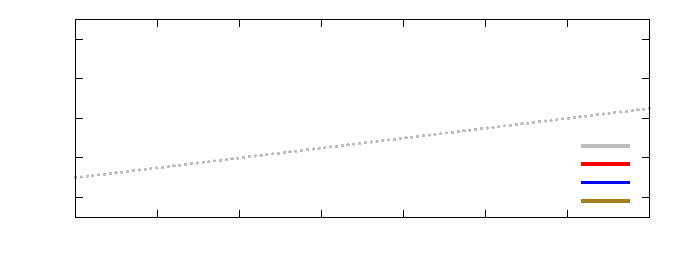
\includegraphics[width={183.00bp},height={169.00bp}]{Quinones}}%
    \gplfronttext
  \end{picture}%
\endgroup

  \caption{Graphical comparison of RI-CC2 methods for quinones. Each point is represented by the compound number given in Table \ref{tab:Quinones}. The dashed line indicates the reference CCSD(T)+E\textsubscript{CBS} values.}
  \label{fig:Quinones}
\end{figure}
  
The performance of EA-EOM-CC2 in calculating the VBS of quinones is benchmarked using a previously established test set of 10 quinones \cite{schulz2018systematic}. The results are summarised in Table \ref{tab:Quinones} and Figure \ref{fig:Quinones}. The table includes experimental adiabatic electron affinities and theoretical CCSD(T)+E\textsubscript{CBS} reference values.\\

Previous studies have demonstrated that CC2 typically performs poorly for VBSs; however, the implementation of spin-component scaling (SCS) corrections markedly enhances the accuracy of CC2 for these states \cite{paran2024performance}. The RI-CC2 results presented here include calculations both with and without SCS corrections, utilising two different basis sets: VTZ (aug-cc-pVTZ) and VDZ (aug-cc-pVDZ).\\

The incorporation of SCS improves the accuracy of CC2 for valence-bound states, corroborating the findings of Ref. \citenum{paran2024performance, shaalan2022accurate}. In general unscaled EA-EOM-RI-CC2 overbinds the electron, and the inclusion of SCS results in a slight underbinding. When comparing the results to experimental data, CC2 might appear to provide better agreement than CCSD. This apparent discrepancy arises because the experimental measurements represent adiabatic electron affinities, whilst the calculations determine vertical electron affinities.\\ 

 As with the case of DBSs, a smaller cardinality leads to a cancellation of errors in the CC2 binding energies, resulting in apparently more exact results (though arising from more inaccurate calculations). Regarding the inclusion of the extremely diffuse functions necessary for modelling DBSs, these have no impact on the VBS energy, indicating that such functions do not contribute to the description of the VBS. Of course, it is still necessary to use augmented basis sets to ensure that the VBS is well described, as the electron density of the VBS is more diffuse than that of the neutral molecule.\\

 It is noteworthy, however, that in all cases, the CC2 method reproduces the correct trend, as illustrated in Figure \ref{fig:Quinones}. The error introduced remains remarkably consistent across different molecules. Subsequent calculations omit SCS, as both DBS and VBS states can be obtained from the same Hamiltonian; one can expect a systematic overbinding of $\mathrm{\sim}$0.2 eV ensuring consistency in the results. It is also important to note that DBS predictions are known to deteriorate significantly when SCS is applied \cite{paran2024performance}, and therefore it is not a desirable method for this work. 

%This is explained by the nature of the DBS; the additional electron is situated far from the core electrons, resulting in a substantially weaker exchange interaction compared to the Coulomb interaction. This characteristic diminishes the effectiveness of SCS for such systems.

\subsection{Photoelectron Cross-section from EOM-CC2/CCSD}\label{sec:results:crosssection}

As a part of this work, Dyson orbitals between EOM-CC2 states have been implemented within the \texttt{ccman2} module of the \textit{Q-Chem} software package. To evaluate their quality, one must go beyond mere visual assessment.\\

Photodetachment cross-sections for 24 valence bound and dipole bound states were calculated using the \textit{ezDyson} package \cite{gozem2022ezspectra,gozem2015photoionization}. These calculations employ orbitals from three different sources: EOM-CC2 Dyson orbitals, EOM-CCSD Dyson orbitals and the dominant Hartree-Fock orbital. The complete results can be found in appendix \ref{ch:appendix:crosssection}. Figure \ref{fig:ezDyson} shows two representative examples: the valence bound state of azulene and the dipole bound state of nitromethane.\\

The results demonstrate  that EOM-CC2 successfully captures the essential features of the cross-section, appearing nearly identical in the case of nitromethane's dipole-bound state and showing only minor deviations for azulene. In contrast, using HF orbitals as approximations for Dyson orbitals fails to reproduce the shape obtained with EOM-CCSD. Although a single HF orbital typically dominates the Dyson orbital \cite{diaz2019dyson}, the contributions from additional electronic configurations introduced by the correlation prove to be significant.

\begin{figure}[th!]
    \centering
    \small
    % GNUPLOT: LaTeX picture with Postscript
\begingroup
  \makeatletter
  \providecommand\color[2][]{%
    \GenericError{(gnuplot) \space\space\space\@spaces}{%
      Package color not loaded in conjunction with
      terminal option `colourtext'%
    }{See the gnuplot documentation for explanation.%
    }{Either use 'blacktext' in gnuplot or load the package
      color.sty in LaTeX.}%
    \renewcommand\color[2][]{}%
  }%
  \providecommand\includegraphics[2][]{%
    \GenericError{(gnuplot) \space\space\space\@spaces}{%
      Package graphicx or graphics not loaded%
    }{See the gnuplot documentation for explanation.%
    }{The gnuplot epslatex terminal needs graphicx.sty or graphics.sty.}%
    \renewcommand\includegraphics[2][]{}%
  }%
  \providecommand\rotatebox[2]{#2}%
  \@ifundefined{ifGPcolor}{%
    \newif\ifGPcolor
    \GPcolortrue
  }{}%
  \@ifundefined{ifGPblacktext}{%
    \newif\ifGPblacktext
    \GPblacktexttrue
  }{}%
  % define a \g@addto@macro without @ in the name:
  \let\gplgaddtomacro\g@addto@macro
  % define empty templates for all commands taking text:
  \gdef\gplbacktext{}%
  \gdef\gplfronttext{}%
  \makeatother
  \ifGPblacktext
    % no textcolor at all
    \def\colorrgb#1{}%
    \def\colorgray#1{}%
  \else
    % gray or color?
    \ifGPcolor
      \def\colorrgb#1{\color[rgb]{#1}}%
      \def\colorgray#1{\color[gray]{#1}}%
      \expandafter\def\csname LTw\endcsname{\color{white}}%
      \expandafter\def\csname LTb\endcsname{\color{black}}%
      \expandafter\def\csname LTa\endcsname{\color{black}}%
      \expandafter\def\csname LT0\endcsname{\color[rgb]{1,0,0}}%
      \expandafter\def\csname LT1\endcsname{\color[rgb]{0,1,0}}%
      \expandafter\def\csname LT2\endcsname{\color[rgb]{0,0,1}}%
      \expandafter\def\csname LT3\endcsname{\color[rgb]{1,0,1}}%
      \expandafter\def\csname LT4\endcsname{\color[rgb]{0,1,1}}%
      \expandafter\def\csname LT5\endcsname{\color[rgb]{1,1,0}}%
      \expandafter\def\csname LT6\endcsname{\color[rgb]{0,0,0}}%
      \expandafter\def\csname LT7\endcsname{\color[rgb]{1,0.3,0}}%
      \expandafter\def\csname LT8\endcsname{\color[rgb]{0.5,0.5,0.5}}%
    \else
      % gray
      \def\colorrgb#1{\color{black}}%
      \def\colorgray#1{\color[gray]{#1}}%
      \expandafter\def\csname LTw\endcsname{\color{white}}%
      \expandafter\def\csname LTb\endcsname{\color{black}}%
      \expandafter\def\csname LTa\endcsname{\color{black}}%
      \expandafter\def\csname LT0\endcsname{\color{black}}%
      \expandafter\def\csname LT1\endcsname{\color{black}}%
      \expandafter\def\csname LT2\endcsname{\color{black}}%
      \expandafter\def\csname LT3\endcsname{\color{black}}%
      \expandafter\def\csname LT4\endcsname{\color{black}}%
      \expandafter\def\csname LT5\endcsname{\color{black}}%
      \expandafter\def\csname LT6\endcsname{\color{black}}%
      \expandafter\def\csname LT7\endcsname{\color{black}}%
      \expandafter\def\csname LT8\endcsname{\color{black}}%
    \fi
  \fi
    \setlength{\unitlength}{0.0500bp}%
    \ifx\gptboxheight\undefined%
      \newlength{\gptboxheight}%
      \newlength{\gptboxwidth}%
      \newsavebox{\gptboxtext}%
    \fi%
    \setlength{\fboxrule}{0.5pt}%
    \setlength{\fboxsep}{1pt}%
    \definecolor{tbcol}{rgb}{1,1,1}%
\begin{picture}(6980.00,3480.00)%
    \gplgaddtomacro\gplbacktext{%
      \csname LTb\endcsname%%
      \put(598,519){\makebox(0,0)[r]{\strut{}$0$}}%
      \csname LTb\endcsname%%
      \put(598,806){\makebox(0,0)[r]{\strut{}$2$}}%
      \csname LTb\endcsname%%
      \put(598,1093){\makebox(0,0)[r]{\strut{}$4$}}%
      \csname LTb\endcsname%%
      \put(598,1380){\makebox(0,0)[r]{\strut{}$6$}}%
      \csname LTb\endcsname%%
      \put(598,1667){\makebox(0,0)[r]{\strut{}$8$}}%
      \csname LTb\endcsname%%
      \put(598,1954){\makebox(0,0)[r]{\strut{}$10$}}%
      \csname LTb\endcsname%%
      \put(598,2242){\makebox(0,0)[r]{\strut{}$12$}}%
      \csname LTb\endcsname%%
      \put(598,2529){\makebox(0,0)[r]{\strut{}$14$}}%
      \csname LTb\endcsname%%
      \put(598,2816){\makebox(0,0)[r]{\strut{}$16$}}%
      \csname LTb\endcsname%%
      \put(598,3103){\makebox(0,0)[r]{\strut{}$18$}}%
      \csname LTb\endcsname%%
      \put(598,3390){\makebox(0,0)[r]{\strut{}$20$}}%
      \csname LTb\endcsname%%
      \put(696,343){\makebox(0,0){\strut{}$0$}}%
      \csname LTb\endcsname%%
      \put(1252,343){\makebox(0,0){\strut{}$2$}}%
      \csname LTb\endcsname%%
      \put(1809,343){\makebox(0,0){\strut{}$4$}}%
      \csname LTb\endcsname%%
      \put(2366,343){\makebox(0,0){\strut{}$6$}}%
      \csname LTb\endcsname%%
      \put(2923,343){\makebox(0,0){\strut{}$8$}}%
      \csname LTb\endcsname%%
      \put(3479,343){\makebox(0,0){\strut{}$10$}}%
    }%
    \gplgaddtomacro\gplfronttext{%
      \csname LTb\endcsname%%
      \put(2790,3135){\makebox(0,0)[r]{\strut{}CC2}}%
      \csname LTb\endcsname%%
      \put(2790,2959){\makebox(0,0)[r]{\strut{}CCSD}}%
      \csname LTb\endcsname%%
      \put(2790,2783){\makebox(0,0)[r]{\strut{}HF}}%
      \csname LTb\endcsname%%
      \put(240,1954){\rotatebox{-270.00}{\makebox(0,0){\strut{}X sec  (a.u.)}}}%
      \csname LTb\endcsname%%
      \put(2087,79){\makebox(0,0){\strut{}$\mathrm{E_I+E_k}$ (eV)}}%
    }%
    \gplgaddtomacro\gplbacktext{%
      \csname LTb\endcsname%%
      \put(3938,519){\makebox(0,0)[r]{\strut{}$0$}}%
      \csname LTb\endcsname%%
      \put(3938,997){\makebox(0,0)[r]{\strut{}$200$}}%
      \csname LTb\endcsname%%
      \put(3938,1476){\makebox(0,0)[r]{\strut{}$400$}}%
      \csname LTb\endcsname%%
      \put(3938,1954){\makebox(0,0)[r]{\strut{}$600$}}%
      \csname LTb\endcsname%%
      \put(3938,2433){\makebox(0,0)[r]{\strut{}$800$}}%
      \csname LTb\endcsname%%
      \put(3938,2912){\makebox(0,0)[r]{\strut{}$1000$}}%
      \csname LTb\endcsname%%
      \put(3938,3390){\makebox(0,0)[r]{\strut{}$1200$}}%
      \csname LTb\endcsname%%
      \put(4036,343){\makebox(0,0){\strut{}$0$}}%
      \csname LTb\endcsname%%
      \put(4732,343){\makebox(0,0){\strut{}$0.5$}}%
      \csname LTb\endcsname%%
      \put(5428,343){\makebox(0,0){\strut{}$1$}}%
      \csname LTb\endcsname%%
      \put(6124,343){\makebox(0,0){\strut{}$1.5$}}%
      \csname LTb\endcsname%%
      \put(6820,343){\makebox(0,0){\strut{}$2$}}%
    }%
    \gplgaddtomacro\gplfronttext{%
      \csname LTb\endcsname%%
      \put(6130,3135){\makebox(0,0)[r]{\strut{}CC2}}%
      \csname LTb\endcsname%%
      \put(6130,2959){\makebox(0,0)[r]{\strut{}CCSD}}%
      \csname LTb\endcsname%%
      \put(6130,2783){\makebox(0,0)[r]{\strut{}HF}}%
      \csname LTb\endcsname%%
      \put(5428,79){\makebox(0,0){\strut{}$\mathrm{E_I+E_k}$ (eV)}}%
    }%
    \gplbacktext
    \put(0,0){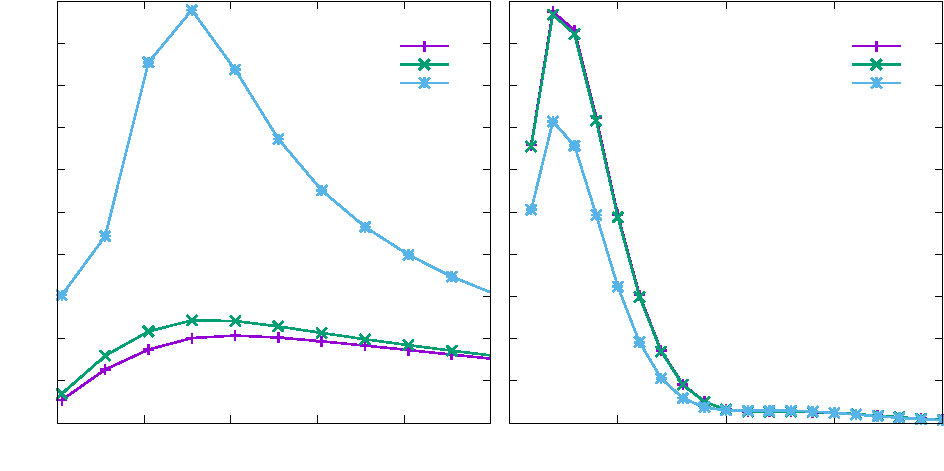
\includegraphics[width={349.00bp},height={174.00bp}]{ezDyson}}%
    \gplfronttext
    \put(1150,1350){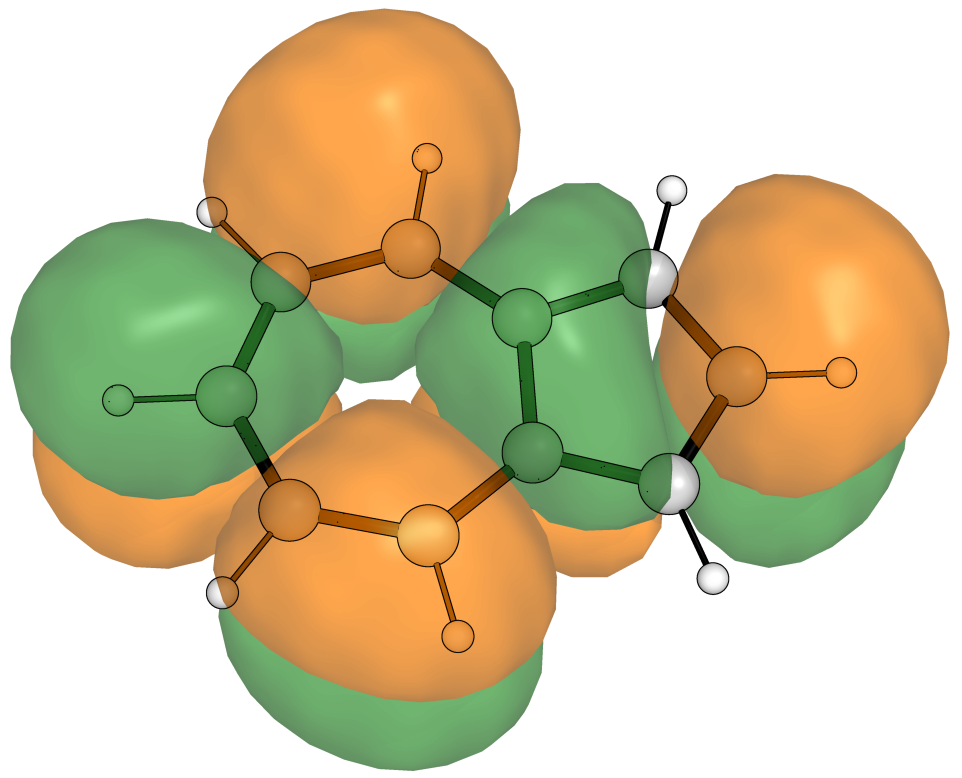
\includegraphics[scale=0.27]{azulene.png}}%
    \put(5100,1300){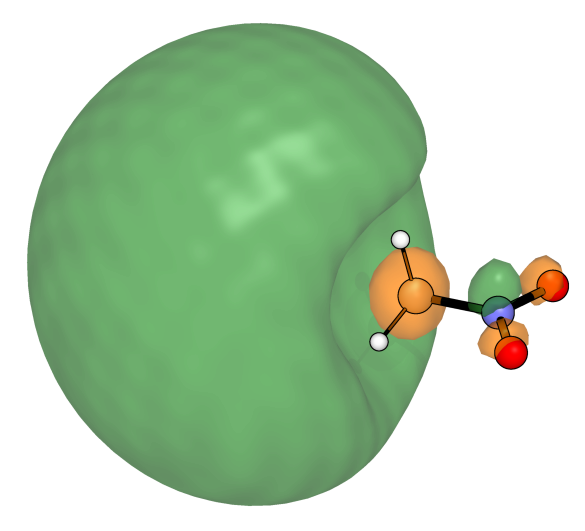
\includegraphics[scale=0.45]{../../introduction/image/MeNO2_DBS.png}}%
  \end{picture}%
\endgroup

    %figsize is set in image/test.gp 
    \caption[Photoedetachment Crossections.]{ Photoedetachment cross-sections of azulene (VBS) and nitromethane (DBS). The cross-sections were calculated using Dyson orbitals from EOM-CC2, EOM-CCSD and the dominant HF orbital in the EOM-CCSD Dyson orbital. The corresponding EA-EOM-CC2 Dyson orbitals are also shown as insets.}
    \label{fig:ezDyson}
\end{figure}

\section{Study on the Anion States of Ubiquinone}

Once the performance of the methods has been assessed, the focus shifts to the anion states of ubiquinone (CoQ). All results presented here are based on the calculations performed with RI-EA-EOM-CC/aug-cc-pVDZ+6s3p unless specified otherwise.

\subsection{Energy and Dipole Surfaces of CoQ}

\subsubsection{Surfaces of Q0}

The conformational landscape of the simplest ubiquinone, Q\textsubscript{0}, was investigated by varying the dihedral angles of the methoxy chains relative to the quinone plane in steps of 20\degree, as shown in Figure \ref{fig:Q0_dyson}. These dihedral angles represent the most significant degrees of freedom in the system, as the remainder of the molecule is relatively rigid. This approach enables the construction of potential energy surfaces (PES), dipole strength surfaces, and PES for the anionic states (VBS and DBS), as depicted in Figure \ref{fig:Q0_maps}. Owing to the C\textsubscript{2} symmetry present when the methoxy chains are coplanar, only half of the surface points require sampling.\\
\begin{figure}[b!]
  \centering
  \begin{minipage}[b]{0.30\textwidth}
    \centering
    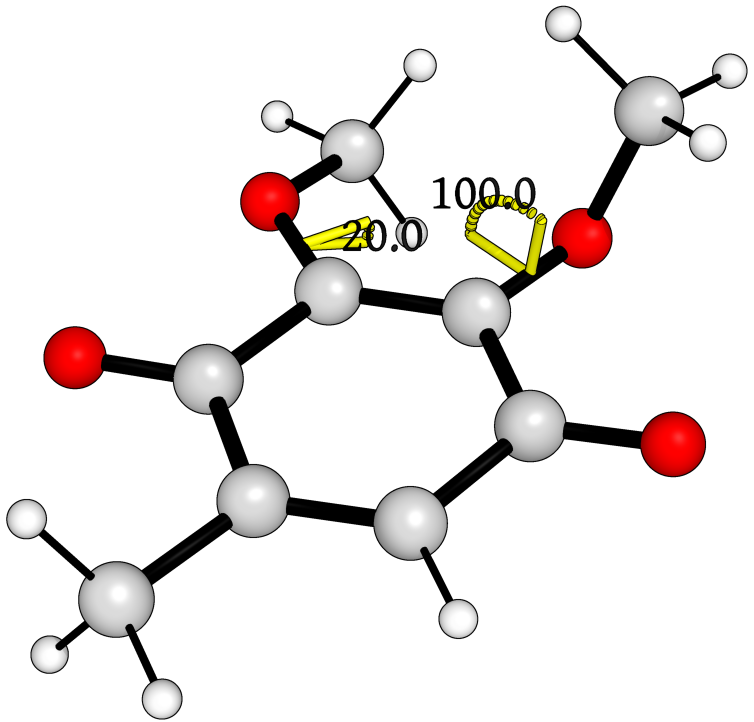
\includegraphics[width=1.15\textwidth]{chapters/results/image/dihedrals.png}
    \vspace{15pt}
    \small\emph{Methoxy dihedrals}
  \end{minipage}
  \hfill
  \begin{minipage}[b]{0.30\textwidth}
    \centering
      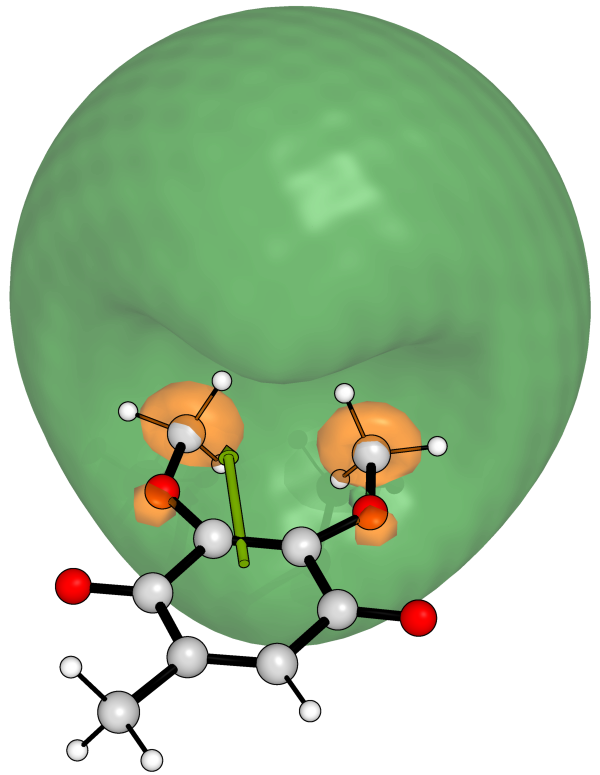
\includegraphics[width=0.8\textwidth]{chapters/results/image/Q0_181.png}
      \small\emph{Region A \\ $(0,0)~\mu=2.5~D$ E=15.8~meV}
  \end{minipage}
  \hfill
  \begin{minipage}[b]{0.30\textwidth}
    \centering
      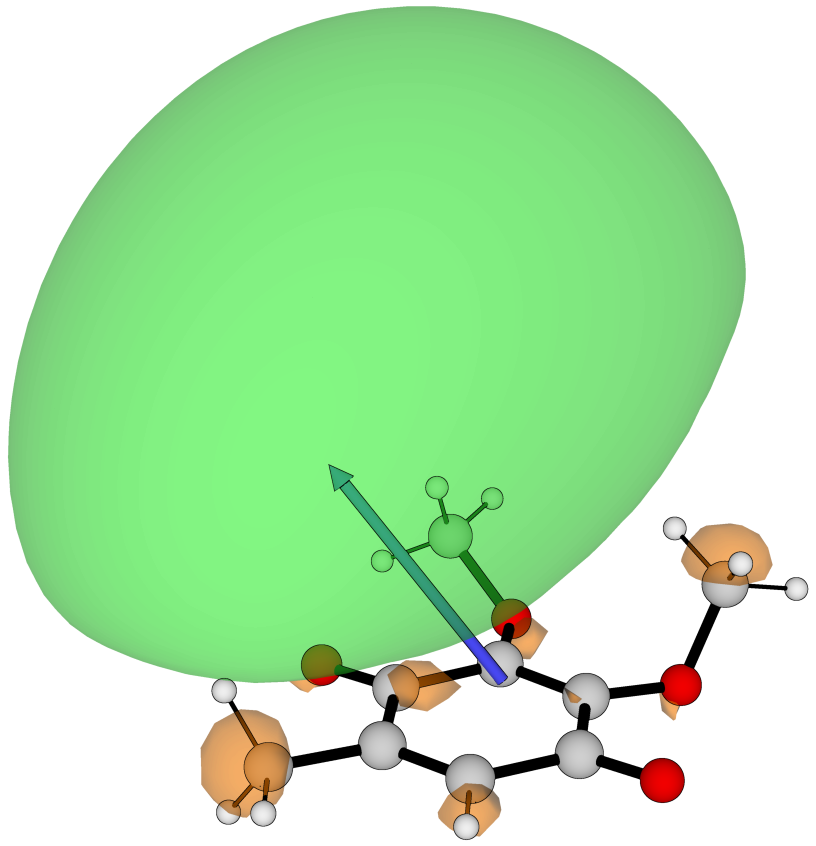
\includegraphics[width=\textwidth]{chapters/results/image/Q0_52.png}
      \small\emph{Region B $(\pm140,\mp20)~\mu=3.2~D$, $E=6.2~meV$}
  \end{minipage}
  \caption[Dyson orbitals of Q0]{Dyson orbitals of Q0 calculated with RI-EA-EOM-CC2/aug-cc-pVDZ+6s3p. The left panel explicitly shows the methoxy dihedral coordinates. The middle panel shows the Dyson orbital of the strongest bound DBS from region B. The right panel shows the Dyson orbital strongest bound DBS from region A. The isosurface is set to 0.005 a.u. and the dipole moment vector is shown as a green arrow with origin at the centre of mass.}
  \label{fig:Q0_dyson}
\end{figure}

\begin{figure}[b!]
  \centering
  \small
  % GNUPLOT: LaTeX picture with Postscript
\begingroup
  \makeatletter
  \providecommand\color[2][]{%
    \GenericError{(gnuplot) \space\space\space\@spaces}{%
      Package color not loaded in conjunction with
      terminal option `colourtext'%
    }{See the gnuplot documentation for explanation.%
    }{Either use 'blacktext' in gnuplot or load the package
      color.sty in LaTeX.}%
    \renewcommand\color[2][]{}%
  }%
  \providecommand\includegraphics[2][]{%
    \GenericError{(gnuplot) \space\space\space\@spaces}{%
      Package graphicx or graphics not loaded%
    }{See the gnuplot documentation for explanation.%
    }{The gnuplot epslatex terminal needs graphicx.sty or graphics.sty.}%
    \renewcommand\includegraphics[2][]{}%
  }%
  \providecommand\rotatebox[2]{#2}%
  \@ifundefined{ifGPcolor}{%
    \newif\ifGPcolor
    \GPcolortrue
  }{}%
  \@ifundefined{ifGPblacktext}{%
    \newif\ifGPblacktext
    \GPblacktexttrue
  }{}%
  % define a \g@addto@macro without @ in the name:
  \let\gplgaddtomacro\g@addto@macro
  % define empty templates for all commands taking text:
  \gdef\gplbacktext{}%
  \gdef\gplfronttext{}%
  \makeatother
  \ifGPblacktext
    % no textcolor at all
    \def\colorrgb#1{}%
    \def\colorgray#1{}%
  \else
    % gray or color?
    \ifGPcolor
      \def\colorrgb#1{\color[rgb]{#1}}%
      \def\colorgray#1{\color[gray]{#1}}%
      \expandafter\def\csname LTw\endcsname{\color{white}}%
      \expandafter\def\csname LTb\endcsname{\color{black}}%
      \expandafter\def\csname LTa\endcsname{\color{black}}%
      \expandafter\def\csname LT0\endcsname{\color[rgb]{1,0,0}}%
      \expandafter\def\csname LT1\endcsname{\color[rgb]{0,1,0}}%
      \expandafter\def\csname LT2\endcsname{\color[rgb]{0,0,1}}%
      \expandafter\def\csname LT3\endcsname{\color[rgb]{1,0,1}}%
      \expandafter\def\csname LT4\endcsname{\color[rgb]{0,1,1}}%
      \expandafter\def\csname LT5\endcsname{\color[rgb]{1,1,0}}%
      \expandafter\def\csname LT6\endcsname{\color[rgb]{0,0,0}}%
      \expandafter\def\csname LT7\endcsname{\color[rgb]{1,0.3,0}}%
      \expandafter\def\csname LT8\endcsname{\color[rgb]{0.5,0.5,0.5}}%
    \else
      % gray
      \def\colorrgb#1{\color{black}}%
      \def\colorgray#1{\color[gray]{#1}}%
      \expandafter\def\csname LTw\endcsname{\color{white}}%
      \expandafter\def\csname LTb\endcsname{\color{black}}%
      \expandafter\def\csname LTa\endcsname{\color{black}}%
      \expandafter\def\csname LT0\endcsname{\color{black}}%
      \expandafter\def\csname LT1\endcsname{\color{black}}%
      \expandafter\def\csname LT2\endcsname{\color{black}}%
      \expandafter\def\csname LT3\endcsname{\color{black}}%
      \expandafter\def\csname LT4\endcsname{\color{black}}%
      \expandafter\def\csname LT5\endcsname{\color{black}}%
      \expandafter\def\csname LT6\endcsname{\color{black}}%
      \expandafter\def\csname LT7\endcsname{\color{black}}%
      \expandafter\def\csname LT8\endcsname{\color{black}}%
    \fi
  \fi
    \setlength{\unitlength}{0.0500bp}%
    \ifx\gptboxheight\undefined%
      \newlength{\gptboxheight}%
      \newlength{\gptboxwidth}%
      \newsavebox{\gptboxtext}%
    \fi%
    \setlength{\fboxrule}{0.5pt}%
    \setlength{\fboxsep}{1pt}%
    \definecolor{tbcol}{rgb}{1,1,1}%
\begin{picture}(9060.00,9060.00)%
    \gplgaddtomacro\gplbacktext{%
    }%
    \gplgaddtomacro\gplfronttext{%
      \csname LTb\endcsname%%
      \put(444,5102){\makebox(0,0)[r]{\strut{}$-160$}}%
      \csname LTb\endcsname%%
      \put(444,5544){\makebox(0,0)[r]{\strut{}$-120$}}%
      \csname LTb\endcsname%%
      \put(444,5986){\makebox(0,0)[r]{\strut{}$-80$}}%
      \csname LTb\endcsname%%
      \put(444,6428){\makebox(0,0)[r]{\strut{}$-40$}}%
      \csname LTb\endcsname%%
      \put(444,6870){\makebox(0,0)[r]{\strut{}$0$}}%
      \csname LTb\endcsname%%
      \put(444,7312){\makebox(0,0)[r]{\strut{}$40$}}%
      \csname LTb\endcsname%%
      \put(444,7754){\makebox(0,0)[r]{\strut{}$80$}}%
      \csname LTb\endcsname%%
      \put(444,8196){\makebox(0,0)[r]{\strut{}$120$}}%
      \csname LTb\endcsname%%
      \put(444,8638){\makebox(0,0)[r]{\strut{}$160$}}%
      \csname LTb\endcsname%%
      \put(542,4705){\makebox(0,0){\strut{}}}%
      \csname LTb\endcsname%%
      \put(1205,4705){\makebox(0,0){\strut{}}}%
      \csname LTb\endcsname%%
      \put(1868,4705){\makebox(0,0){\strut{}}}%
      \csname LTb\endcsname%%
      \put(2531,4705){\makebox(0,0){\strut{}}}%
      \csname LTb\endcsname%%
      \put(3194,4705){\makebox(0,0){\strut{}}}%
      \csname LTb\endcsname%%
      \put(3857,4705){\makebox(0,0){\strut{}}}%
      \csname LTb\endcsname%%
      \put(4520,4705){\makebox(0,0){\strut{}}}%
      \csname LTb\endcsname%%
      \put(87,6870){\rotatebox{-270.00}{\makebox(0,0){\normalsize $\Psi$}}}%
      \csname LTb\endcsname%%
      \put(2089,7154){\rotatebox{-66.00}{\makebox(0,0){\strut{}\textcolor{black}{\footnotesize 500}}}}%
      \csname LTb\endcsname%%
      \put(2907,6987){\rotatebox{130.00}{\makebox(0,0){\strut{}\textcolor{black}{\footnotesize 400}}}}%
      \csname LTb\endcsname%%
      \put(2146,6682){\rotatebox{-27.00}{\makebox(0,0){\strut{}\textcolor{black}{\footnotesize 400}}}}%
      \csname LTb\endcsname%%
      \put(2313,7650){\rotatebox{154.00}{\makebox(0,0){\strut{}\textcolor{black}{\footnotesize 300}}}}%
      \csname LTb\endcsname%%
      \put(2302,6385){\rotatebox{-39.00}{\makebox(0,0){\strut{}\textcolor{black}{\footnotesize 300}}}}%
      \csname LTb\endcsname%%
      \put(3383,6779){\rotatebox{113.00}{\makebox(0,0){\strut{}\textcolor{black}{\footnotesize 200}}}}%
      \csname LTb\endcsname%%
      \put(1472,8023){\rotatebox{-143.00}{\makebox(0,0){\strut{}\textcolor{black}{\footnotesize 200}}}}%
      \csname LTb\endcsname%%
      \put(2514,6042){\rotatebox{-26.00}{\makebox(0,0){\strut{}\textcolor{black}{\footnotesize 200}}}}%
      \csname LTb\endcsname%%
      \put(1231,8224){\rotatebox{39.00}{\makebox(0,0){\strut{}\textcolor{black}{\footnotesize 100}}}}%
      \csname LTb\endcsname%%
      \put(3216,8239){\rotatebox{42.00}{\makebox(0,0){\strut{}\textcolor{black}{\footnotesize 100}}}}%
      \csname LTb\endcsname%%
      \put(3517,6877){\rotatebox{-71.00}{\makebox(0,0){\strut{}\textcolor{black}{\footnotesize 100}}}}%
      \csname LTb\endcsname%%
      \put(1307,7421){\rotatebox{-43.00}{\makebox(0,0){\strut{}\textcolor{black}{\footnotesize 100}}}}%
      \csname LTb\endcsname%%
      \put(1378,5563){\rotatebox{-33.00}{\makebox(0,0){\strut{}\textcolor{black}{\footnotesize 100}}}}%
      \csname LTb\endcsname%%
      \put(3383,5294){\rotatebox{-28.00}{\makebox(0,0){\strut{}\textcolor{black}{\footnotesize 100}}}}%
      \csname LTb\endcsname%%
      \put(705,7288){\rotatebox{-112.00}{\makebox(0,0){\strut{}\textcolor{black}{\footnotesize 50}}}}%
      \csname LTb\endcsname%%
      \put(3758,7221){\rotatebox{-149.00}{\makebox(0,0){\strut{}\textcolor{black}{\footnotesize 50}}}}%
      \csname LTb\endcsname%%
      \put(2213,8126){\rotatebox{-28.00}{\makebox(0,0){\strut{}\textcolor{black}{\footnotesize 50}}}}%
      \csname LTb\endcsname%%
      \put(2292,5650){\rotatebox{31.00}{\makebox(0,0){\strut{}\textcolor{black}{\footnotesize 50}}}}%
      \csname LTb\endcsname%%
      \put(2531,8982){\makebox(0,0){\strut{}Conformational Energy (meV)}}%
    }%
    \gplgaddtomacro\gplbacktext{%
    }%
    \gplgaddtomacro\gplfronttext{%
      \csname LTb\endcsname%%
      \put(4874,5102){\makebox(0,0)[r]{\strut{}}}%
      \csname LTb\endcsname%%
      \put(4874,5544){\makebox(0,0)[r]{\strut{}}}%
      \csname LTb\endcsname%%
      \put(4874,5986){\makebox(0,0)[r]{\strut{}}}%
      \csname LTb\endcsname%%
      \put(4874,6428){\makebox(0,0)[r]{\strut{}}}%
      \csname LTb\endcsname%%
      \put(4874,6870){\makebox(0,0)[r]{\strut{}}}%
      \csname LTb\endcsname%%
      \put(4874,7312){\makebox(0,0)[r]{\strut{}}}%
      \csname LTb\endcsname%%
      \put(4874,7754){\makebox(0,0)[r]{\strut{}}}%
      \csname LTb\endcsname%%
      \put(4874,8196){\makebox(0,0)[r]{\strut{}}}%
      \csname LTb\endcsname%%
      \put(4874,8638){\makebox(0,0)[r]{\strut{}}}%
      \csname LTb\endcsname%%
      \put(4971,4705){\makebox(0,0){\strut{}}}%
      \csname LTb\endcsname%%
      \put(5634,4705){\makebox(0,0){\strut{}}}%
      \csname LTb\endcsname%%
      \put(6297,4705){\makebox(0,0){\strut{}}}%
      \csname LTb\endcsname%%
      \put(6960,4705){\makebox(0,0){\strut{}}}%
      \csname LTb\endcsname%%
      \put(7623,4705){\makebox(0,0){\strut{}}}%
      \csname LTb\endcsname%%
      \put(8286,4705){\makebox(0,0){\strut{}}}%
      \csname LTb\endcsname%%
      \put(8949,4705){\makebox(0,0){\strut{}}}%
      \csname LTb\endcsname%%
      \put(5031,7851){\rotatebox{37.00}{\makebox(0,0){\strut{}\textcolor{black}{\footnotesize 3.0}}}}%
      \csname LTb\endcsname%%
      \put(8832,6500){\rotatebox{156.00}{\makebox(0,0){\strut{}\textcolor{black}{\footnotesize 3.0}}}}%
      \csname LTb\endcsname%%
      \put(6547,7260){\rotatebox{-78.00}{\makebox(0,0){\strut{}\textcolor{black}{\footnotesize 2.5}}}}%
      \csname LTb\endcsname%%
      \put(5651,8271){\rotatebox{-7.00}{\makebox(0,0){\strut{}\textcolor{black}{\footnotesize 2.5}}}}%
      \csname LTb\endcsname%%
      \put(5409,6940){\rotatebox{-127.00}{\makebox(0,0){\strut{}\textcolor{black}{\footnotesize 2.5}}}}%
      \csname LTb\endcsname%%
      \put(8618,7519){\rotatebox{-88.00}{\makebox(0,0){\strut{}\textcolor{black}{\footnotesize 2.5}}}}%
      \csname LTb\endcsname%%
      \put(8083,6140){\rotatebox{-101.00}{\makebox(0,0){\strut{}\textcolor{black}{\footnotesize 2.5}}}}%
      \csname LTb\endcsname%%
      \put(5500,6320){\rotatebox{91.00}{\makebox(0,0){\strut{}\textcolor{black}{\footnotesize 2.0}}}}%
      \csname LTb\endcsname%%
      \put(6314,7040){\rotatebox{-47.00}{\makebox(0,0){\strut{}\textcolor{black}{\footnotesize 2.0}}}}%
      \csname LTb\endcsname%%
      \put(7233,6000){\rotatebox{-38.00}{\makebox(0,0){\strut{}\textcolor{black}{\footnotesize 2.0}}}}%
      \csname LTb\endcsname%%
      \put(6531,7999){\rotatebox{-101.00}{\makebox(0,0){\strut{}\textcolor{black}{\footnotesize 2.0}}}}%
      \csname LTb\endcsname%%
      \put(7425,6960){\rotatebox{-59.00}{\makebox(0,0){\strut{}\textcolor{black}{\footnotesize 2.0}}}}%
      \csname LTb\endcsname%%
      \put(8359,7080){\rotatebox{64.00}{\makebox(0,0){\strut{}\textcolor{black}{\footnotesize 2.0}}}}%
      \csname LTb\endcsname%%
      \put(5471,5690){\rotatebox{52.00}{\makebox(0,0){\strut{}\textcolor{black}{\footnotesize 1.5}}}}%
      \csname LTb\endcsname%%
      \put(6291,6706){\rotatebox{-17.00}{\makebox(0,0){\strut{}\textcolor{black}{\footnotesize 1.5}}}}%
      \csname LTb\endcsname%%
      \put(6870,5426){\rotatebox{-106.00}{\makebox(0,0){\strut{}\textcolor{black}{\footnotesize 1.5}}}}%
      \csname LTb\endcsname%%
      \put(7650,8582){\rotatebox{-176.00}{\makebox(0,0){\strut{}\textcolor{black}{\footnotesize 1.5}}}}%
      \csname LTb\endcsname%%
      \put(7238,7519){\rotatebox{-45.00}{\makebox(0,0){\strut{}\textcolor{black}{\footnotesize 1.5}}}}%
      \csname LTb\endcsname%%
      \put(8205,7420){\rotatebox{78.00}{\makebox(0,0){\strut{}\textcolor{black}{\footnotesize 1.5}}}}%
      \csname LTb\endcsname%%
      \put(5771,5854){\rotatebox{56.00}{\makebox(0,0){\strut{}\textcolor{black}{\footnotesize 1.0}}}}%
      \csname LTb\endcsname%%
      \put(6570,5482){\rotatebox{-124.00}{\makebox(0,0){\strut{}\textcolor{black}{\footnotesize 1.0}}}}%
      \csname LTb\endcsname%%
      \put(7490,8350){\rotatebox{-162.00}{\makebox(0,0){\strut{}\textcolor{black}{\footnotesize 1.0}}}}%
      \csname LTb\endcsname%%
      \put(8062,7739){\rotatebox{60.00}{\makebox(0,0){\strut{}\textcolor{black}{\footnotesize 1.0}}}}%
      \csname LTb\endcsname%%
      \put(5883,5721){\rotatebox{-132.00}{\makebox(0,0){\strut{}\textcolor{black}{\footnotesize 0.5}}}}%
      \csname LTb\endcsname%%
      \put(7669,8179){\rotatebox{-140.00}{\makebox(0,0){\strut{}\textcolor{black}{\footnotesize 0.5}}}}%
      \csname LTb\endcsname%%
      \put(6960,8982){\makebox(0,0){Dipole Strength (Debye)}}%
    }%
    \gplgaddtomacro\gplbacktext{%
    }%
    \gplgaddtomacro\gplfronttext{%
      \csname LTb\endcsname%%
      \put(444,763){\makebox(0,0)[r]{\strut{}$-160$}}%
      \csname LTb\endcsname%%
      \put(444,1205){\makebox(0,0)[r]{\strut{}$-120$}}%
      \csname LTb\endcsname%%
      \put(444,1647){\makebox(0,0)[r]{\strut{}$-80$}}%
      \csname LTb\endcsname%%
      \put(444,2089){\makebox(0,0)[r]{\strut{}$-40$}}%
      \csname LTb\endcsname%%
      \put(444,2531){\makebox(0,0)[r]{\strut{}$0$}}%
      \csname LTb\endcsname%%
      \put(444,2973){\makebox(0,0)[r]{\strut{}$40$}}%
      \csname LTb\endcsname%%
      \put(444,3415){\makebox(0,0)[r]{\strut{}$80$}}%
      \csname LTb\endcsname%%
      \put(444,3857){\makebox(0,0)[r]{\strut{}$120$}}%
      \csname LTb\endcsname%%
      \put(444,4298){\makebox(0,0)[r]{\strut{}$160$}}%
      \csname LTb\endcsname%%
      \put(542,366){\makebox(0,0){\strut{}$-180$}}%
      \csname LTb\endcsname%%
      \put(1205,366){\makebox(0,0){\strut{}$-120$}}%
      \csname LTb\endcsname%%
      \put(1868,366){\makebox(0,0){\strut{}$-60$}}%
      \csname LTb\endcsname%%
      \put(2531,366){\makebox(0,0){\strut{}$0$}}%
      \csname LTb\endcsname%%
      \put(3194,366){\makebox(0,0){\strut{}$60$}}%
      \csname LTb\endcsname%%
      \put(3857,366){\makebox(0,0){\strut{}$120$}}%
      \csname LTb\endcsname%%
      \put(4519,366){\makebox(0,0){\strut{}$180$}}%
      \csname LTb\endcsname%%
      \put(87,2531){\rotatebox{-270.00}{\makebox(0,0){\normalsize $\Psi$}}}%
      \csname LTb\endcsname%%
      \put(2531,102){\makebox(0,0){\normalsize $\Phi$}}%
      \csname LTb\endcsname%%
      \put(2390,2781){\rotatebox{150.00}{\makebox(0,0){\strut{}\textcolor{black}{\footnotesize 1.3}}}}%
      \csname LTb\endcsname%%
      \put(2270,2355){\rotatebox{-57.00}{\makebox(0,0){\strut{}\textcolor{black}{\footnotesize 1.4}}}}%
      \csname LTb\endcsname%%
      \put(2912,2859){\rotatebox{124.00}{\makebox(0,0){\strut{}\textcolor{black}{\footnotesize 1.5}}}}%
      \csname LTb\endcsname%%
      \put(2511,1819){\rotatebox{-36.00}{\makebox(0,0){\strut{}\textcolor{black}{\footnotesize 1.5}}}}%
      \csname LTb\endcsname%%
      \put(2052,3555){\rotatebox{51.00}{\makebox(0,0){\strut{}\textcolor{black}{\footnotesize 1.6}}}}%
      \csname LTb\endcsname%%
      \put(2164,1627){\rotatebox{-79.00}{\makebox(0,0){\strut{}\textcolor{black}{\footnotesize 1.6}}}}%
      \csname LTb\endcsname%%
      \put(3435,2928){\rotatebox{-15.00}{\makebox(0,0){\strut{}\textcolor{black}{\footnotesize 1.6}}}}%
      \csname LTb\endcsname%%
      \put(3530,2028){\rotatebox{40.00}{\makebox(0,0){\strut{}\textcolor{black}{\footnotesize 1.6}}}}%
      \csname LTb\endcsname%%
      \put(1814,1426){\rotatebox{-81.00}{\makebox(0,0){\strut{}\textcolor{black}{\footnotesize 1.7}}}}%
      \csname LTb\endcsname%%
      \put(1753,3676){\rotatebox{49.00}{\makebox(0,0){\strut{}\textcolor{black}{\footnotesize 1.7}}}}%
      \csname LTb\endcsname%%
      \put(3475,3295){\rotatebox{-26.00}{\makebox(0,0){\strut{}\textcolor{black}{\footnotesize 1.7}}}}%
      \csname LTb\endcsname%%
      \put(3592,1667){\rotatebox{55.00}{\makebox(0,0){\strut{}\textcolor{black}{\footnotesize 1.7}}}}%
      \csname LTb\endcsname%%
      \put(2531,4643){\makebox(0,0){VBA EA (eV)}}%
    }%
    \gplgaddtomacro\gplbacktext{%
    }%
    \gplgaddtomacro\gplfronttext{%
      \csname LTb\endcsname%%
      \put(4874,763){\makebox(0,0)[r]{\strut{}}}%
      \csname LTb\endcsname%%
      \put(4874,1205){\makebox(0,0)[r]{\strut{}}}%
      \csname LTb\endcsname%%
      \put(4874,1647){\makebox(0,0)[r]{\strut{}}}%
      \csname LTb\endcsname%%
      \put(4874,2089){\makebox(0,0)[r]{\strut{}}}%
      \csname LTb\endcsname%%
      \put(4874,2531){\makebox(0,0)[r]{\strut{}}}%
      \csname LTb\endcsname%%
      \put(4874,2973){\makebox(0,0)[r]{\strut{}}}%
      \csname LTb\endcsname%%
      \put(4874,3415){\makebox(0,0)[r]{\strut{}}}%
      \csname LTb\endcsname%%
      \put(4874,3857){\makebox(0,0)[r]{\strut{}}}%
      \csname LTb\endcsname%%
      \put(4874,4298){\makebox(0,0)[r]{\strut{}}}%
      \csname LTb\endcsname%%
      \put(4971,366){\makebox(0,0){\strut{}$-180$}}%
      \csname LTb\endcsname%%
      \put(5634,366){\makebox(0,0){\strut{}$-120$}}%
      \csname LTb\endcsname%%
      \put(6297,366){\makebox(0,0){\strut{}$-60$}}%
      \csname LTb\endcsname%%
      \put(6960,366){\makebox(0,0){\strut{}$0$}}%
      \csname LTb\endcsname%%
      \put(7623,366){\makebox(0,0){\strut{}$60$}}%
      \csname LTb\endcsname%%
      \put(8286,366){\makebox(0,0){\strut{}$120$}}%
      \csname LTb\endcsname%%
      \put(8949,366){\makebox(0,0){\strut{}$180$}}%
      \csname LTb\endcsname%%
      \put(6960,102){\makebox(0,0){\normalsize $\Phi$}}%
      \csname LTb\endcsname%%
      \put(7021,2310){\rotatebox{-43.00}{\makebox(0,0){\strut{}\textcolor{black}{\footnotesize 12}}}}%
      \csname LTb\endcsname%%
      \put(7236,2069){\rotatebox{-30.00}{\makebox(0,0){\strut{}\textcolor{black}{\footnotesize 9}}}}%
      \csname LTb\endcsname%%
      \put(5255,3234){\rotatebox{-53.00}{\makebox(0,0){\strut{}\textcolor{black}{\footnotesize 6}}}}%
      \csname LTb\endcsname%%
      \put(7107,2792){\rotatebox{130.00}{\makebox(0,0){\strut{}\textcolor{black}{\footnotesize 6}}}}%
      \csname LTb\endcsname%%
      \put(7422,1854){\rotatebox{-23.00}{\makebox(0,0){\strut{}\textcolor{black}{\footnotesize 6}}}}%
      \csname LTb\endcsname%%
      \put(8467,1607){\rotatebox{-42.00}{\makebox(0,0){\strut{}\textcolor{black}{\footnotesize 6}}}}%
      \csname LTb\endcsname%%
      \put(7686,2189){\rotatebox{113.00}{\makebox(0,0){\strut{}\textcolor{black}{\footnotesize 3}}}}%
      \csname LTb\endcsname%%
      \put(5496,3877){\rotatebox{-170.00}{\makebox(0,0){\strut{}\textcolor{black}{\footnotesize 3}}}}%
      \csname LTb\endcsname%%
      \put(6531,2591){\rotatebox{-35.00}{\makebox(0,0){\strut{}\textcolor{black}{\footnotesize 3}}}}%
      \csname LTb\endcsname%%
      \put(8748,1369){\rotatebox{50.00}{\makebox(0,0){\strut{}\textcolor{black}{\footnotesize 3}}}}%
      \csname LTb\endcsname%%
      \put(5107,1627){\rotatebox{-108.00}{\makebox(0,0){\strut{}\textcolor{black}{\footnotesize 0}}}}%
      \csname LTb\endcsname%%
      \put(8798,2912){\rotatebox{-74.00}{\makebox(0,0){\strut{}\textcolor{black}{\footnotesize 0}}}}%
      \csname LTb\endcsname%%
      \put(6538,3598){\rotatebox{-62.00}{\makebox(0,0){\strut{}\textcolor{black}{\footnotesize 0}}}}%
      \csname LTb\endcsname%%
      \put(8748,2534){\rotatebox{3.00}{\makebox(0,0){\strut{}\textcolor{black}{\footnotesize 0}}}}%
      \csname LTb\endcsname%%
      \put(6568,2390){\rotatebox{-68.00}{\makebox(0,0){\strut{}\textcolor{black}{\footnotesize 0}}}}%
      \csname LTb\endcsname%%
      \put(8788,1198){\rotatebox{47.00}{\makebox(0,0){\strut{}\textcolor{black}{\footnotesize 0}}}}%
      \csname LTb\endcsname%%
      \put(5767,2531){\makebox(0,0){\strut{}\textcolor{black}{\normalsize \textbf{B}}}}%
      \csname LTb\endcsname%%
      \put(8153,2531){\makebox(0,0){\strut{}\textcolor{black}{\normalsize \textbf{B}}}}%
      \csname LTb\endcsname%%
      \put(6483,2133){\makebox(0,0){\strut{}\textcolor{black}{\normalsize \textbf{A}}}}%
      \csname LTb\endcsname%%
      \put(6960,4643){\makebox(0,0){DBA EA (meV)}}%
    }%
    \gplbacktext
    \put(0,0){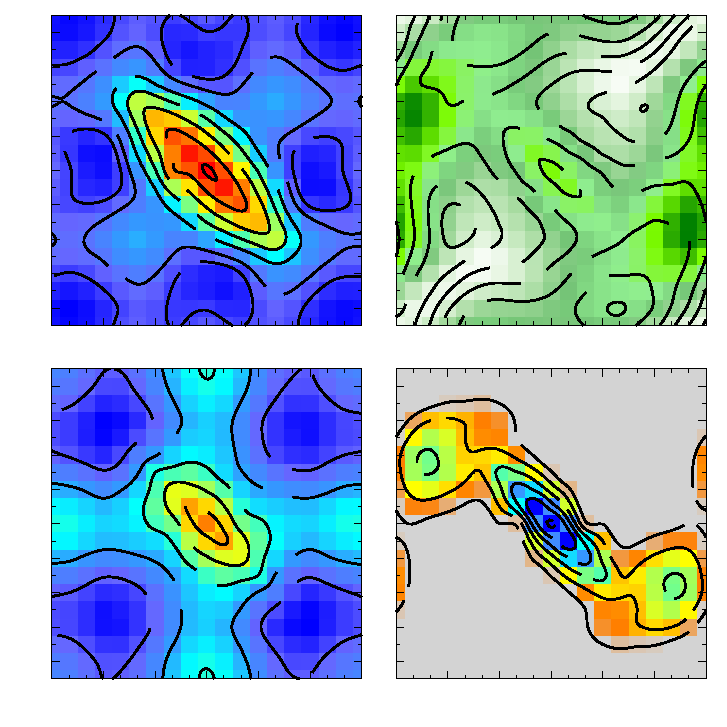
\includegraphics[width={453.00bp},height={453.00bp}]{chapters/results/image/Q0_maps}}%
    \gplfronttext
  \end{picture}%
\endgroup
 
  \caption[Surfaces of Q0]{Surfaces of Q0. From left to right and top to bottom: potential energy surface (CC2), dipole strength surface (DFT TPSS), PES for the VBS (EA-EOM-CC2), and PES for the DBS (EA-EOM-CC2). Gray points the DBS surface indicate that the DBS is not predicted to exist.\label{fig:Q0_maps}}
\end{figure}

The conformational energy surface of the neutral molecule reveals five minima, corresponding to configurations where the methoxy groups are oriented away from each other. The global minimum occurs at (180,180), where both chains are coplanar with the quinone and directed oppositely. Four additional minima are found at $\mathrm{(\pm140,\mp20)}$ and $\mathrm{(\pm20,\mp140)}$, each approximately 10 meV above the global minimum. The presence of a methyl group at position 5 slightly perturbs the symmetry between the methoxy chains, but its influence on the energy landscape is minimal due to its spatial separation. The energy barriers separating these wells range from 65 to 100 meV, suggesting that interconversion between conformers is feasible at ambient temperature. A pronounced steric repulsion is observed near (0,0), where both methoxy chains are coplanar and oriented towards each other, resulting in an energy penalty of approximately 580 meV.\\

The dipole strength surface largely reflects the vector sum of the individual methoxy group dipoles. When both chains are aligned in the same direction, the dipole strength is maximised, and vice versa. The lowest dipole moment, below 0.5 Debye, is found near (180,180). Local maxima in dipole strength are observed at (0,0) with a strength of 2.5 D, and $\mathrm{(\pm160,\mp80)}$ ($\mu=3.2$~D), $\mathrm{(\pm60,\mp160)}$ ($\mu=3.4$~D), and $\mathrm{(\pm80,\pm180)}$ ($\mu=3.2$~D), with the latter two coinciding with conformational minima at $\mathrm{(\pm140,\mp20)}$.\\

The valence-bound state (VBS) surface can be rationalised by considering the electron-withdrawing effect of out-of-plane methoxy groups and the electron-donating effect of in-plane conjugation. The VBS minimum is observed at four points where both chains are approximately $\pm120\degree$ out of plane, with a vertical electron affinity (VAE) of 1.77~eV. Notably, when either chain is coplanar ($\pm0\degree$), the VAE increases by about 0.2~eV. The global minimum occurs at (0,0), where both chains are in-plane, with a VAE of 1.26~eV. The pronounced dependence of the electron affinity on methoxy conformation has been proposed as a mechanism to control the electron transfer processes in quinone redox enzymes\cite{schulz2018systematic,nonella1998quantum,taguchi2013tuning,taguchi2013conformational,deAlmeida2014effect}.\label{sec:Q0_maps}\\

The dipole-bound state (DBS) surface, as anticipated, closely follows the dipole strength surface. It is important to note that in regions where the DBS is unbound, the EA-EOM-CC2 binding energies are not physically meaningful and would approach zero in the basis set limit. Three distinct regions are apparent, mirroring those of the dipole strength surface. The region at $\mathrm{(\pm60,\pm180)}$ ($\mu=3.1$~D) is the smallest and most weakly bound, with only five points exhibiting binding energies up to 2 meV. Region B in Figure \ref{fig:Q0_maps}, centred at $\mathrm{(\pm140,\mp20)}$ ($\mu=3.2$~D), is larger and reaches a maximum binding energy of 6.2 meV. Region A, at (0,0), is the most strongly bound, with a maximum of 15.8 meV, despite its lower dipole strength. This may be attributed to the orientation of the dipole moment: in region B, the dipole points above the quinone, and the DBS electron density  interacts repulsively with the \textpi system, whereas in region A, the dipole is directed away from the quinone plane. In Figure \ref{fig:Q0_dyson}, these cases are shown.\\

Surprisingly, CC2 predicts DBSs in region A supported by dipole moments as small as 1.6D, which is significantly lower than the commonly cited threshold of 2.5D and falls within the range of the ideal dipole DBS \cite{jordan2003theory}. This result suggests that, in addition to the excess electron density being spatially separated from the valence electrons, further stabilisation arises from dispersion interactions with the $\pi$ system. Effects similar to this have been experimentally observed in indolide anions\cite{yuan2023observation}. Nevertheless, the high conformational energy of region A makes its population unlikely.\\

\subsubsection{Surfaces of Q1}

The isoprene tail introduces additional degrees of freedom, resulting in a more complex conformational landscape. To investigate its effect, the analogous surfaces for Q\textsubscript{1} were constructed by fixing the bend and dihedral angles of the isoprene unit relative to the quinone plane. The frozen values of said angles were taken from the crystal structure of the quinone in the active site of bacterial complex I (PDB: 6I0D) \cite{gutierrez2020key}, as presented in Figure \ref{fig:Q1_dyson}. The results are shown in Figure \ref{fig:Q1_maps}. In this case, the molecule has no plane of symmetry and all points of the surface have to be sampled. The PES and dipole surfaces were calculated with DFT using the TPSS functional. Due to the computational cost, only the points with a dipole strength above 1.6 Debye were sampled.\\

 \begin{figure}[ht!]
  \centering
  \small
  % GNUPLOT: LaTeX picture with Postscript
\begingroup
  \makeatletter
  \providecommand\color[2][]{%
    \GenericError{(gnuplot) \space\space\space\@spaces}{%
      Package color not loaded in conjunction with
      terminal option `colourtext'%
    }{See the gnuplot documentation for explanation.%
    }{Either use 'blacktext' in gnuplot or load the package
      color.sty in LaTeX.}%
    \renewcommand\color[2][]{}%
  }%
  \providecommand\includegraphics[2][]{%
    \GenericError{(gnuplot) \space\space\space\@spaces}{%
      Package graphicx or graphics not loaded%
    }{See the gnuplot documentation for explanation.%
    }{The gnuplot epslatex terminal needs graphicx.sty or graphics.sty.}%
    \renewcommand\includegraphics[2][]{}%
  }%
  \providecommand\rotatebox[2]{#2}%
  \@ifundefined{ifGPcolor}{%
    \newif\ifGPcolor
    \GPcolortrue
  }{}%
  \@ifundefined{ifGPblacktext}{%
    \newif\ifGPblacktext
    \GPblacktexttrue
  }{}%
  % define a \g@addto@macro without @ in the name:
  \let\gplgaddtomacro\g@addto@macro
  % define empty templates for all commands taking text:
  \gdef\gplbacktext{}%
  \gdef\gplfronttext{}%
  \makeatother
  \ifGPblacktext
    % no textcolor at all
    \def\colorrgb#1{}%
    \def\colorgray#1{}%
  \else
    % gray or color?
    \ifGPcolor
      \def\colorrgb#1{\color[rgb]{#1}}%
      \def\colorgray#1{\color[gray]{#1}}%
      \expandafter\def\csname LTw\endcsname{\color{white}}%
      \expandafter\def\csname LTb\endcsname{\color{black}}%
      \expandafter\def\csname LTa\endcsname{\color{black}}%
      \expandafter\def\csname LT0\endcsname{\color[rgb]{1,0,0}}%
      \expandafter\def\csname LT1\endcsname{\color[rgb]{0,1,0}}%
      \expandafter\def\csname LT2\endcsname{\color[rgb]{0,0,1}}%
      \expandafter\def\csname LT3\endcsname{\color[rgb]{1,0,1}}%
      \expandafter\def\csname LT4\endcsname{\color[rgb]{0,1,1}}%
      \expandafter\def\csname LT5\endcsname{\color[rgb]{1,1,0}}%
      \expandafter\def\csname LT6\endcsname{\color[rgb]{0,0,0}}%
      \expandafter\def\csname LT7\endcsname{\color[rgb]{1,0.3,0}}%
      \expandafter\def\csname LT8\endcsname{\color[rgb]{0.5,0.5,0.5}}%
    \else
      % gray
      \def\colorrgb#1{\color{black}}%
      \def\colorgray#1{\color[gray]{#1}}%
      \expandafter\def\csname LTw\endcsname{\color{white}}%
      \expandafter\def\csname LTb\endcsname{\color{black}}%
      \expandafter\def\csname LTa\endcsname{\color{black}}%
      \expandafter\def\csname LT0\endcsname{\color{black}}%
      \expandafter\def\csname LT1\endcsname{\color{black}}%
      \expandafter\def\csname LT2\endcsname{\color{black}}%
      \expandafter\def\csname LT3\endcsname{\color{black}}%
      \expandafter\def\csname LT4\endcsname{\color{black}}%
      \expandafter\def\csname LT5\endcsname{\color{black}}%
      \expandafter\def\csname LT6\endcsname{\color{black}}%
      \expandafter\def\csname LT7\endcsname{\color{black}}%
      \expandafter\def\csname LT8\endcsname{\color{black}}%
    \fi
  \fi
    \setlength{\unitlength}{0.0500bp}%
    \ifx\gptboxheight\undefined%
      \newlength{\gptboxheight}%
      \newlength{\gptboxwidth}%
      \newsavebox{\gptboxtext}%
    \fi%
    \setlength{\fboxrule}{0.5pt}%
    \setlength{\fboxsep}{1pt}%
    \definecolor{tbcol}{rgb}{1,1,1}%
\begin{picture}(6980.00,6980.00)%
    \gplgaddtomacro\gplbacktext{%
    }%
    \gplgaddtomacro\gplfronttext{%
      \csname LTb\endcsname%%
      \put(389,3994){\makebox(0,0)[r]{\strut{}$-160$}}%
      \csname LTb\endcsname%%
      \put(389,4326){\makebox(0,0)[r]{\strut{}$-120$}}%
      \csname LTb\endcsname%%
      \put(389,4659){\makebox(0,0)[r]{\strut{}$-80$}}%
      \csname LTb\endcsname%%
      \put(389,4991){\makebox(0,0)[r]{\strut{}$-40$}}%
      \csname LTb\endcsname%%
      \put(389,5324){\makebox(0,0)[r]{\strut{}$0$}}%
      \csname LTb\endcsname%%
      \put(389,5656){\makebox(0,0)[r]{\strut{}$40$}}%
      \csname LTb\endcsname%%
      \put(389,5989){\makebox(0,0)[r]{\strut{}$80$}}%
      \csname LTb\endcsname%%
      \put(389,6321){\makebox(0,0)[r]{\strut{}$120$}}%
      \csname LTb\endcsname%%
      \put(389,6654){\makebox(0,0)[r]{\strut{}$160$}}%
      \csname LTb\endcsname%%
      \put(487,3652){\makebox(0,0){\strut{}}}%
      \csname LTb\endcsname%%
      \put(986,3652){\makebox(0,0){\strut{}}}%
      \csname LTb\endcsname%%
      \put(1484,3652){\makebox(0,0){\strut{}}}%
      \csname LTb\endcsname%%
      \put(1983,3652){\makebox(0,0){\strut{}}}%
      \csname LTb\endcsname%%
      \put(2482,3652){\makebox(0,0){\strut{}}}%
      \csname LTb\endcsname%%
      \put(2981,3652){\makebox(0,0){\strut{}}}%
      \csname LTb\endcsname%%
      \put(3480,3652){\makebox(0,0){\strut{}}}%
      \csname LTb\endcsname%%
      \put(32,5324){\rotatebox{-270.00}{\makebox(0,0){\normalsize $\Psi$}}}%
      \csname LTb\endcsname%%
      \put(1669,5498){\rotatebox{-63.00}{\makebox(0,0){\strut{}\textcolor{black}{\footnotesize 500}}}}%
      \csname LTb\endcsname%%
      \put(2272,5409){\rotatebox{130.00}{\makebox(0,0){\strut{}\textcolor{black}{\footnotesize 400}}}}%
      \csname LTb\endcsname%%
      \put(1758,5160){\rotatebox{-46.00}{\makebox(0,0){\strut{}\textcolor{black}{\footnotesize 400}}}}%
      \csname LTb\endcsname%%
      \put(1725,5940){\rotatebox{157.00}{\makebox(0,0){\strut{}\textcolor{black}{\footnotesize 300}}}}%
      \csname LTb\endcsname%%
      \put(1870,4897){\rotatebox{-39.00}{\makebox(0,0){\strut{}\textcolor{black}{\footnotesize 300}}}}%
      \csname LTb\endcsname%%
      \put(2641,5261){\rotatebox{115.00}{\makebox(0,0){\strut{}\textcolor{black}{\footnotesize 200}}}}%
      \csname LTb\endcsname%%
      \put(1191,6171){\rotatebox{-140.00}{\makebox(0,0){\strut{}\textcolor{black}{\footnotesize 200}}}}%
      \csname LTb\endcsname%%
      \put(1989,4683){\rotatebox{-24.00}{\makebox(0,0){\strut{}\textcolor{black}{\footnotesize 200}}}}%
      \csname LTb\endcsname%%
      \put(1191,4995){\rotatebox{39.00}{\makebox(0,0){\strut{}\textcolor{black}{\footnotesize 100}}}}%
      \csname LTb\endcsname%%
      \put(1142,6544){\rotatebox{44.00}{\makebox(0,0){\strut{}\textcolor{black}{\footnotesize 100}}}}%
      \csname LTb\endcsname%%
      \put(2474,6418){\rotatebox{62.00}{\makebox(0,0){\strut{}\textcolor{black}{\footnotesize 100}}}}%
      \csname LTb\endcsname%%
      \put(2748,5336){\rotatebox{-73.00}{\makebox(0,0){\strut{}\textcolor{black}{\footnotesize 100}}}}%
      \csname LTb\endcsname%%
      \put(990,4433){\rotatebox{-33.00}{\makebox(0,0){\strut{}\textcolor{black}{\footnotesize 100}}}}%
      \csname LTb\endcsname%%
      \put(2588,4180){\rotatebox{-44.00}{\makebox(0,0){\strut{}\textcolor{black}{\footnotesize 100}}}}%
      \csname LTb\endcsname%%
      \put(585,5638){\rotatebox{-104.00}{\makebox(0,0){\strut{}\textcolor{black}{\footnotesize 50}}}}%
      \csname LTb\endcsname%%
      \put(1865,6569){\rotatebox{158.00}{\makebox(0,0){\strut{}\textcolor{black}{\footnotesize 50}}}}%
      \csname LTb\endcsname%%
      \put(1541,3978){\rotatebox{-72.00}{\makebox(0,0){\strut{}\textcolor{black}{\footnotesize 50}}}}%
      \csname LTb\endcsname%%
      \put(2926,5567){\rotatebox{-139.00}{\makebox(0,0){\strut{}\textcolor{black}{\footnotesize 50}}}}%
      \csname LTb\endcsname%%
      \put(1983,6943){\makebox(0,0){\strut{}Conformational Energy (meV)}}%
    }%
    \gplgaddtomacro\gplbacktext{%
    }%
    \gplgaddtomacro\gplfronttext{%
      \csname LTb\endcsname%%
      \put(3695,3994){\makebox(0,0)[r]{\strut{}}}%
      \csname LTb\endcsname%%
      \put(3695,4326){\makebox(0,0)[r]{\strut{}}}%
      \csname LTb\endcsname%%
      \put(3695,4659){\makebox(0,0)[r]{\strut{}}}%
      \csname LTb\endcsname%%
      \put(3695,4991){\makebox(0,0)[r]{\strut{}}}%
      \csname LTb\endcsname%%
      \put(3695,5324){\makebox(0,0)[r]{\strut{}}}%
      \csname LTb\endcsname%%
      \put(3695,5656){\makebox(0,0)[r]{\strut{}}}%
      \csname LTb\endcsname%%
      \put(3695,5989){\makebox(0,0)[r]{\strut{}}}%
      \csname LTb\endcsname%%
      \put(3695,6321){\makebox(0,0)[r]{\strut{}}}%
      \csname LTb\endcsname%%
      \put(3695,6654){\makebox(0,0)[r]{\strut{}}}%
      \csname LTb\endcsname%%
      \put(3793,3652){\makebox(0,0){\strut{}}}%
      \csname LTb\endcsname%%
      \put(4291,3652){\makebox(0,0){\strut{}}}%
      \csname LTb\endcsname%%
      \put(4790,3652){\makebox(0,0){\strut{}}}%
      \csname LTb\endcsname%%
      \put(5289,3652){\makebox(0,0){\strut{}}}%
      \csname LTb\endcsname%%
      \put(5788,3652){\makebox(0,0){\strut{}}}%
      \csname LTb\endcsname%%
      \put(6287,3652){\makebox(0,0){\strut{}}}%
      \csname LTb\endcsname%%
      \put(6785,3652){\makebox(0,0){\strut{}}}%
      \csname LTb\endcsname%%
      \put(5700,4218){\rotatebox{43.00}{\makebox(0,0){\strut{}\textcolor{black}{\footnotesize 3.0}}}}%
      \csname LTb\endcsname%%
      \put(5522,5222){\rotatebox{129.00}{\makebox(0,0){\strut{}\textcolor{black}{\footnotesize 2.5}}}}%
      \csname LTb\endcsname%%
      \put(4353,6459){\rotatebox{-72.00}{\makebox(0,0){\strut{}\textcolor{black}{\footnotesize 2.5}}}}%
      \csname LTb\endcsname%%
      \put(5372,6661){\makebox(0,0){\strut{}\textcolor{black}{\footnotesize 2.5}}}%
      \csname LTb\endcsname%%
      \put(4515,3989){\rotatebox{40.00}{\makebox(0,0){\strut{}\textcolor{black}{\footnotesize 2.5}}}}%
      \csname LTb\endcsname%%
      \put(5552,4386){\rotatebox{42.00}{\makebox(0,0){\strut{}\textcolor{black}{\footnotesize 2.5}}}}%
      \csname LTb\endcsname%%
      \put(6545,4794){\rotatebox{-22.00}{\makebox(0,0){\strut{}\textcolor{black}{\footnotesize 2.5}}}}%
      \csname LTb\endcsname%%
      \put(4187,6670){\rotatebox{-108.00}{\makebox(0,0){\strut{}\textcolor{black}{\footnotesize 2.0}}}}%
      \csname LTb\endcsname%%
      \put(4560,6009){\rotatebox{-4.00}{\makebox(0,0){\strut{}\textcolor{black}{\footnotesize 2.0}}}}%
      \csname LTb\endcsname%%
      \put(5567,6455){\rotatebox{-5.00}{\makebox(0,0){\strut{}\textcolor{black}{\footnotesize 2.0}}}}%
      \csname LTb\endcsname%%
      \put(5101,4265){\rotatebox{24.00}{\makebox(0,0){\strut{}\textcolor{black}{\footnotesize 2.0}}}}%
      \csname LTb\endcsname%%
      \put(5251,5011){\rotatebox{145.00}{\makebox(0,0){\strut{}\textcolor{black}{\footnotesize 2.0}}}}%
      \csname LTb\endcsname%%
      \put(5086,5696){\rotatebox{-23.00}{\makebox(0,0){\strut{}\textcolor{black}{\footnotesize 2.0}}}}%
      \csname LTb\endcsname%%
      \put(5973,5109){\rotatebox{-19.00}{\makebox(0,0){\strut{}\textcolor{black}{\footnotesize 2.0}}}}%
      \csname LTb\endcsname%%
      \put(4006,5346){\rotatebox{50.00}{\makebox(0,0){\strut{}\textcolor{black}{\footnotesize 1.5}}}}%
      \csname LTb\endcsname%%
      \put(4845,5166){\rotatebox{-50.00}{\makebox(0,0){\strut{}\textcolor{black}{\footnotesize 1.5}}}}%
      \csname LTb\endcsname%%
      \put(4906,4402){\rotatebox{-173.00}{\makebox(0,0){\strut{}\textcolor{black}{\footnotesize 1.5}}}}%
      \csname LTb\endcsname%%
      \put(6065,6324){\rotatebox{-155.00}{\makebox(0,0){\strut{}\textcolor{black}{\footnotesize 1.5}}}}%
      \csname LTb\endcsname%%
      \put(5236,5857){\rotatebox{-36.00}{\makebox(0,0){\strut{}\textcolor{black}{\footnotesize 1.5}}}}%
      \csname LTb\endcsname%%
      \put(6199,5401){\rotatebox{16.00}{\makebox(0,0){\strut{}\textcolor{black}{\footnotesize 1.5}}}}%
      \csname LTb\endcsname%%
      \put(3907,4143){\rotatebox{75.00}{\makebox(0,0){\strut{}\textcolor{black}{\footnotesize 1.0}}}}%
      \csname LTb\endcsname%%
      \put(4274,5214){\rotatebox{14.00}{\makebox(0,0){\strut{}\textcolor{black}{\footnotesize 1.0}}}}%
      \csname LTb\endcsname%%
      \put(4620,4529){\rotatebox{-156.00}{\makebox(0,0){\strut{}\textcolor{black}{\footnotesize 1.0}}}}%
      \csname LTb\endcsname%%
      \put(6003,6130){\rotatebox{-158.00}{\makebox(0,0){\strut{}\textcolor{black}{\footnotesize 1.0}}}}%
      \csname LTb\endcsname%%
      \put(6214,5602){\rotatebox{11.00}{\makebox(0,0){\strut{}\textcolor{black}{\footnotesize 1.0}}}}%
      \csname LTb\endcsname%%
      \put(4533,4880){\rotatebox{116.00}{\makebox(0,0){\strut{}\textcolor{black}{\footnotesize 0.5}}}}%
      \csname LTb\endcsname%%
      \put(5289,6943){\makebox(0,0){Dipole Strength (Debye)}}%
    }%
    \gplgaddtomacro\gplbacktext{%
    }%
    \gplgaddtomacro\gplfronttext{%
      \csname LTb\endcsname%%
      \put(389,723){\makebox(0,0)[r]{\strut{}$-160$}}%
      \csname LTb\endcsname%%
      \put(389,1055){\makebox(0,0)[r]{\strut{}$-120$}}%
      \csname LTb\endcsname%%
      \put(389,1388){\makebox(0,0)[r]{\strut{}$-80$}}%
      \csname LTb\endcsname%%
      \put(389,1720){\makebox(0,0)[r]{\strut{}$-40$}}%
      \csname LTb\endcsname%%
      \put(389,2053){\makebox(0,0)[r]{\strut{}$0$}}%
      \csname LTb\endcsname%%
      \put(389,2385){\makebox(0,0)[r]{\strut{}$40$}}%
      \csname LTb\endcsname%%
      \put(389,2718){\makebox(0,0)[r]{\strut{}$80$}}%
      \csname LTb\endcsname%%
      \put(389,3050){\makebox(0,0)[r]{\strut{}$120$}}%
      \csname LTb\endcsname%%
      \put(389,3383){\makebox(0,0)[r]{\strut{}$160$}}%
      \csname LTb\endcsname%%
      \put(487,380){\makebox(0,0){\strut{}$-180$}}%
      \csname LTb\endcsname%%
      \put(986,380){\makebox(0,0){\strut{}$-120$}}%
      \csname LTb\endcsname%%
      \put(1484,380){\makebox(0,0){\strut{}$-60$}}%
      \csname LTb\endcsname%%
      \put(1983,380){\makebox(0,0){\strut{}$0$}}%
      \csname LTb\endcsname%%
      \put(2482,380){\makebox(0,0){\strut{}$60$}}%
      \csname LTb\endcsname%%
      \put(2981,380){\makebox(0,0){\strut{}$120$}}%
      \csname LTb\endcsname%%
      \put(3479,380){\makebox(0,0){\strut{}$180$}}%
      \csname LTb\endcsname%%
      \put(32,2053){\rotatebox{-270.00}{\makebox(0,0){\normalsize $\Psi$}}}%
      \csname LTb\endcsname%%
      \put(1983,117){\makebox(0,0){\normalsize $\Phi$}}%
      \csname LTb\endcsname%%
      \put(1881,2279){\rotatebox{148.00}{\makebox(0,0){\strut{}\textcolor{black}{\footnotesize 1.3}}}}%
      \csname LTb\endcsname%%
      \put(1696,1928){\rotatebox{-45.00}{\makebox(0,0){\strut{}\textcolor{black}{\footnotesize 1.4}}}}%
      \csname LTb\endcsname%%
      \put(2297,2279){\rotatebox{143.00}{\makebox(0,0){\strut{}\textcolor{black}{\footnotesize 1.5}}}}%
      \csname LTb\endcsname%%
      \put(1947,1554){\rotatebox{-45.00}{\makebox(0,0){\strut{}\textcolor{black}{\footnotesize 1.5}}}}%
      \csname LTb\endcsname%%
      \put(1582,2824){\rotatebox{45.00}{\makebox(0,0){\strut{}\textcolor{black}{\footnotesize 1.6}}}}%
      \csname LTb\endcsname%%
      \put(2693,1629){\rotatebox{48.00}{\makebox(0,0){\strut{}\textcolor{black}{\footnotesize 1.6}}}}%
      \csname LTb\endcsname%%
      \put(883,2824){\rotatebox{-34.00}{\makebox(0,0){\strut{}\textcolor{black}{\footnotesize 1.7}}}}%
      \csname LTb\endcsname%%
      \put(1411,1040){\rotatebox{112.00}{\makebox(0,0){\strut{}\textcolor{black}{\footnotesize 1.7}}}}%
      \csname LTb\endcsname%%
      \put(2845,3372){\rotatebox{-135.00}{\makebox(0,0){\strut{}\textcolor{black}{\footnotesize 1.7}}}}%
      \csname LTb\endcsname%%
      \put(2754,783){\rotatebox{-25.00}{\makebox(0,0){\strut{}\textcolor{black}{\footnotesize 1.7}}}}%
      \csname LTb\endcsname%%
      \put(1983,3672){\makebox(0,0){VBA EA (eV)}}%
    }%
    \gplgaddtomacro\gplbacktext{%
    }%
    \gplgaddtomacro\gplfronttext{%
      \csname LTb\endcsname%%
      \put(3695,723){\makebox(0,0)[r]{\strut{}}}%
      \csname LTb\endcsname%%
      \put(3695,1055){\makebox(0,0)[r]{\strut{}}}%
      \csname LTb\endcsname%%
      \put(3695,1388){\makebox(0,0)[r]{\strut{}}}%
      \csname LTb\endcsname%%
      \put(3695,1720){\makebox(0,0)[r]{\strut{}}}%
      \csname LTb\endcsname%%
      \put(3695,2053){\makebox(0,0)[r]{\strut{}}}%
      \csname LTb\endcsname%%
      \put(3695,2385){\makebox(0,0)[r]{\strut{}}}%
      \csname LTb\endcsname%%
      \put(3695,2718){\makebox(0,0)[r]{\strut{}}}%
      \csname LTb\endcsname%%
      \put(3695,3050){\makebox(0,0)[r]{\strut{}}}%
      \csname LTb\endcsname%%
      \put(3695,3383){\makebox(0,0)[r]{\strut{}}}%
      \csname LTb\endcsname%%
      \put(3793,380){\makebox(0,0){\strut{}$-180$}}%
      \csname LTb\endcsname%%
      \put(4291,380){\makebox(0,0){\strut{}$-120$}}%
      \csname LTb\endcsname%%
      \put(4790,380){\makebox(0,0){\strut{}$-60$}}%
      \csname LTb\endcsname%%
      \put(5289,380){\makebox(0,0){\strut{}$0$}}%
      \csname LTb\endcsname%%
      \put(5788,380){\makebox(0,0){\strut{}$60$}}%
      \csname LTb\endcsname%%
      \put(6287,380){\makebox(0,0){\strut{}$120$}}%
      \csname LTb\endcsname%%
      \put(6785,380){\makebox(0,0){\strut{}$180$}}%
      \csname LTb\endcsname%%
      \put(5289,117){\makebox(0,0){\normalsize $\Phi$}}%
      \csname LTb\endcsname%%
      \put(5528,1735){\rotatebox{-34.00}{\makebox(0,0){\strut{}\textcolor{black}{\footnotesize 9}}}}%
      \csname LTb\endcsname%%
      \put(5878,726){\rotatebox{-22.00}{\makebox(0,0){\strut{}\textcolor{black}{\footnotesize 9}}}}%
      \csname LTb\endcsname%%
      \put(5637,1104){\rotatebox{69.00}{\makebox(0,0){\strut{}\textcolor{black}{\footnotesize 6}}}}%
      \csname LTb\endcsname%%
      \put(5502,2068){\rotatebox{-38.00}{\makebox(0,0){\strut{}\textcolor{black}{\footnotesize 6}}}}%
      \csname LTb\endcsname%%
      \put(6181,648){\rotatebox{-151.00}{\makebox(0,0){\strut{}\textcolor{black}{\footnotesize 6}}}}%
      \csname LTb\endcsname%%
      \put(4831,3035){\rotatebox{39.00}{\makebox(0,0){\strut{}\textcolor{black}{\footnotesize 3}}}}%
      \csname LTb\endcsname%%
      \put(5576,1294){\rotatebox{70.00}{\makebox(0,0){\strut{}\textcolor{black}{\footnotesize 3}}}}%
      \csname LTb\endcsname%%
      \put(5516,2146){\rotatebox{-39.00}{\makebox(0,0){\strut{}\textcolor{black}{\footnotesize 3}}}}%
      \csname LTb\endcsname%%
      \put(6392,679){\rotatebox{-131.00}{\makebox(0,0){\strut{}\textcolor{black}{\footnotesize 3}}}}%
      \csname LTb\endcsname%%
      \put(6108,3458){\rotatebox{24.00}{\makebox(0,0){\strut{}\textcolor{black}{\footnotesize 3}}}}%
      \csname LTb\endcsname%%
      \put(5126,3337){\rotatebox{91.00}{\makebox(0,0){\strut{}\textcolor{black}{\footnotesize 1}}}}%
      \csname LTb\endcsname%%
      \put(6211,3433){\rotatebox{28.00}{\makebox(0,0){\strut{}\textcolor{black}{\footnotesize 1}}}}%
      \csname LTb\endcsname%%
      \put(5332,1584){\rotatebox{128.00}{\makebox(0,0){\strut{}\textcolor{black}{\footnotesize 1}}}}%
      \csname LTb\endcsname%%
      \put(5592,2159){\rotatebox{-34.00}{\makebox(0,0){\strut{}\textcolor{black}{\footnotesize 1}}}}%
      \csname LTb\endcsname%%
      \put(6497,707){\rotatebox{-116.00}{\makebox(0,0){\strut{}\textcolor{black}{\footnotesize 1}}}}%
      \csname LTb\endcsname%%
      \put(4242,2502){\makebox(0,0){\strut{}\textcolor{black}{\normalsize \textbf{C}}}}%
      \csname LTb\endcsname%%
      \put(6336,1963){\makebox(0,0){\strut{}\textcolor{black}{\normalsize \textbf{B}}}}%
      \csname LTb\endcsname%%
      \put(4930,1753){\makebox(0,0){\strut{}\textcolor{black}{\normalsize \textbf{A}}}}%
      \csname LTb\endcsname%%
      \put(5289,3672){\makebox(0,0){DBA EA (meV)}}%
    }%
    \gplbacktext
    \put(0,0){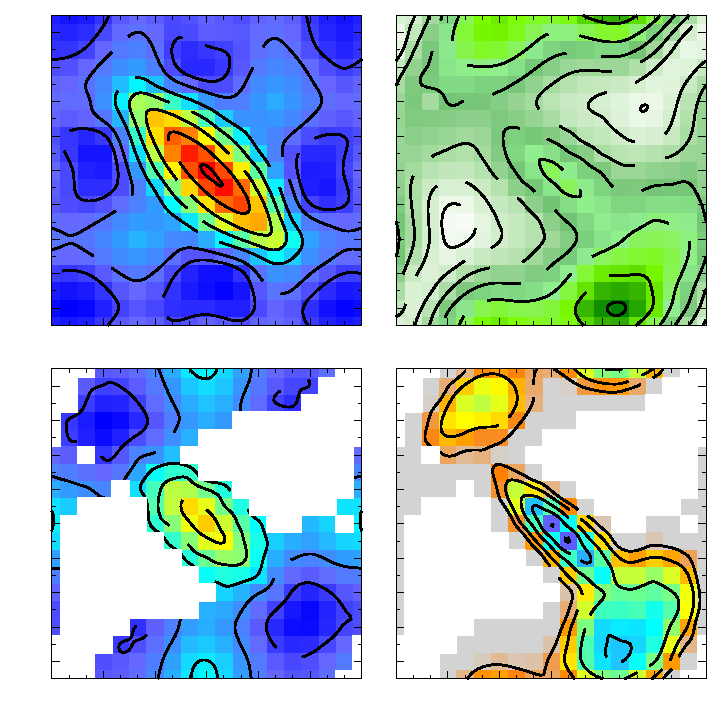
\includegraphics[width={349.00bp},height={349.00bp}]{Q1_maps}}%
    \gplfronttext
  \end{picture}%
\endgroup

  \caption[Surfaces of Q1]{Surfaces of Q1. From left to right and top to bottom: potential energy surface (CC2), dipole strength surface (DFT TPSS), PES for the VBS (EA-EOM-CC2), and PES for the DBS (EA-EOM-CC2). White points in VBS and DBS surfaces were not sampled, and gray points the DBS surface indicate that the DBS is not predicted to exist. \label{fig:Q1_maps}}
\end{figure}

Concerning the conformational potential energy surface (PES), the fixed position of the isoprene tail, distant from the quinone moiety, prevents interaction with the methoxy chains. This renders the scenario largely analogous to that of Q\textsubscript{0}. Steric hindrances would be anticipated with longer tails or alternative configurations. However, the relevance of this particular system is questionable, as crystallographic data \cite{taguchi2013conformational} indicate that the isoprene tail does not penetrate the quinone moiety's pocket. Within a protein, the orientation of the methoxy chains is dictated by the local environment, with specific configurations favoured by interactions with first-shell amino acids.\\

The interpretation of the dipole strength surface is also similar to that of Q\textsubscript{0}, with the addition of a fixed dipole originating from the isoprene group, which is oriented approximately out of the plane. This has the effect of dividing region B from Figure \ref{fig:Q0_maps} into two distinct regions for Q\textsubscript{1}, designated B and C. In region B, the local dipole of the isoprene aligns with the methoxy dipoles, resulting in a maximum dipole strength of 3.3 Debye at (160,-80). Conversely, in region C, destructive interference occurs between the local dipoles, leading to a maximum dipole strength of 2.9 Debye at (-60,160). Region A is only slightly affected, retaining a maximum dipole strength of 2.6 D at (0,0).\\

The VBS surface of Q\textsubscript{1} is more challenging to interpret due to the omitted data points. Nevertheless, the overall picture appears to remain consistent, as the qualitative effect of the rotation of the chains (acting as electron donor or acceptor) is unchanged. The range of vertical electron affinity (VEA) varies surprisingly little, with a global minimum of 1.26 eV at (0,0) and a maximum of 1.76 eV at (-120,120). It had been previously proposed that, contrary to its established spectator role, the isoprene tail might contribute to the stabilisation of the excess electron \cite{pshenichnyuk2020ionizing}. However, the results presented herein suggest that the isoprene tail does not significantly affect the VBS of Q\textsubscript{1}, at least in the conformation employed in this study.\\

Regarding the DBS surface, the impact of the isoprene tail is more pronounced. In region B, where the local dipole of the isoprene tail aligns with the methoxy dipoles, the region expands to encompass a larger area and exhibits a maximum binding energy of 9.1 meV at (80,-160). In region C, the local dipoles interfere destructively, resulting in a smaller area with a maximum binding energy of 5.0 meV at (-80,140). Region A shows a minor difference, with a maximum binding energy of 12.2 meV at (20,-20). In Figure \ref{fig:Q1_dyson}, the Dyson orbitals of the structures are shown. The variations in electron binding energy in regions B and C can be attributed to changes in the dipole moment strength. The alteration in region A, however, is likely related to a decrease in the favourable interactions between the DBS and the rest of the electronic density, as the dipole moment remains largely unchanged. Similarly to the case with Q0, it is noteworthy that structures with dipole moments below 2.5 D are predicted to be bound by EA-EOM-CC2; for example, with dihedrals of (20,20) and a dipole moment of 1.81 D, the binding energy is 2.2 meV.\\

\begin{figure}[h]
  \centering
    \begin{minipage}[b]{0.30\textwidth}
    \centering
      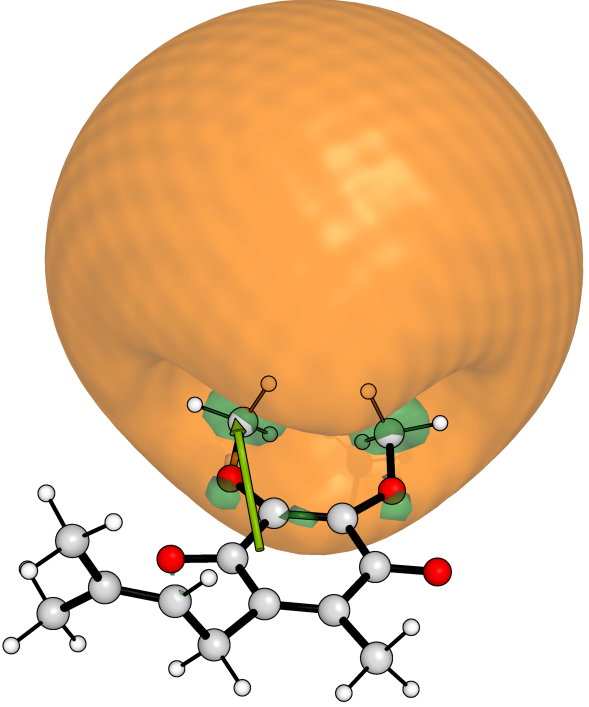
\includegraphics[width=1\textwidth]{chapters/results/image/Q1_199.png}
      \small\emph{Region A \\$(0,0)~\mu=2.6~D$ E=12.2~meV}
  \end{minipage}
  \hfill
  \begin{minipage}[b]{0.30\textwidth}
    \centering
      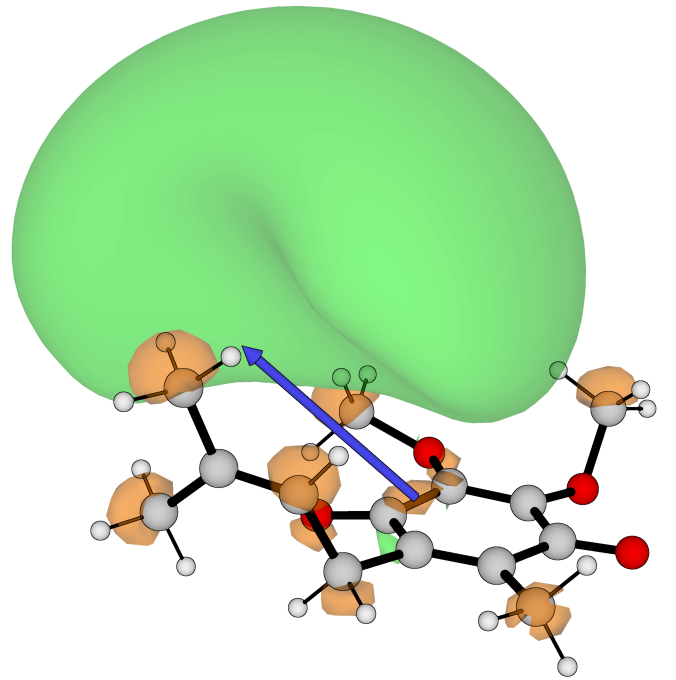
\includegraphics[width=\textwidth]{chapters/results/image/Q1_249.png}
      \small\emph{Region B \\$(160,-80)~\mu=3.3~D$, $E=9.1~meV$}
  \end{minipage}
  \hfill
  \begin{minipage}[b]{0.30\textwidth}
    \centering
    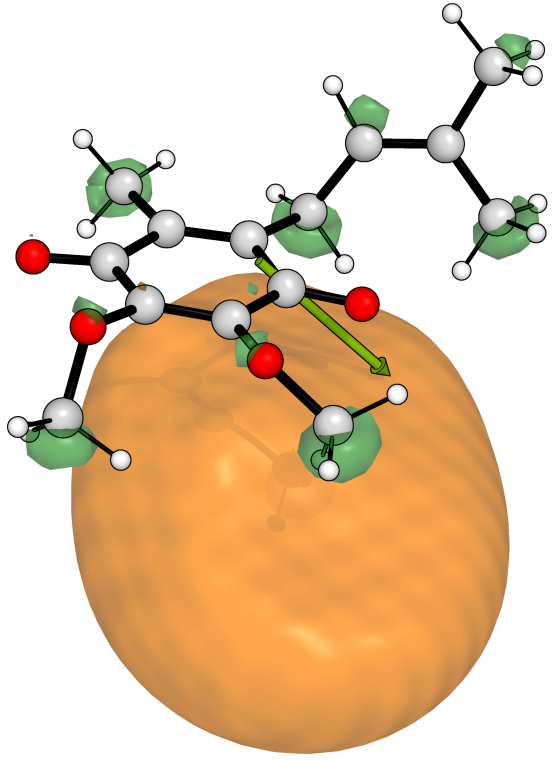
\includegraphics[width=0.9\textwidth]{chapters/results/image/Q1_112.png}
    \small\emph{Region C \\$(-60,160)~\mu=2.9~D$, $E=5.0~meV$}
  \end{minipage}
  \caption[Dyson orbitals of Q1]{Dyson orbitals of Q0 calculated with RI-EA-EOM-CC2/aug-cc-pVDZ+6s3p. The left panel shows the Dyson orbital of the strongest bound DBS from region A. The middle panel shows the Dyson orbital of the strongest bound DBS from region B. The right panel shows the Dyson orbital of the strongest bound DBS from region A. The isosurface is set to 0.005 a.u. and the dipole moment vector is shown as a blue arrow with origin at the centre of mass.}
  \label{fig:Q1_dyson}
\end{figure}

An important consideration for dipole-bound states (DBS) is the extent of correlation between their binding energy and the strength of the dipole moment that supports them. The DBS maps for Q\textsubscript{0}, Figure \ref{fig:Q0_maps}, and Q\textsubscript{1}, Figure \ref{fig:Q1_maps}, are clearly demarcated into distinct regions. Figure \ref{fig:D_vsDBS} presents a scatter plot illustrating all bound points for both Q\textsubscript{0} and Q\textsubscript{1}. This plot demonstrates that the different regions identified in the maps correspond to separate populations in the scatter plot. A correlation between dipole strength and binding energy is observed in all regions, though the degree of this correlation varies. For instance, region A, which accommodates the strongest dipoles, exhibits a nearly linear relationship between these two parameters for both quinones. This could be interepreted as the molecule acting as an ideal dipole. When comparing region A in Q\textsubscript{0} and Q\textsubscript{1}, the slope for Q\textsubscript{0} is steeper than that for Q\textsubscript{1}, indicating that variations in the chemical environment affect the interplay between the dipole moment and the binding strength.\\

Concerning the populations in regions B and C, the relationship between the dipole moment and binding energy is considerably less pronounced. This is likely because the DBS occupies a spatial region closer to the other electrons, specifically the \textpi\ system. In this system, alterations in dipole strength arise from changes in its orientation. Consequently, the displacement of the DBS that accompanies the strengthening of the dipole might result in a less favourable interaction with the remaining electronic density.
In general, the electron binding energy is only loosely correlated with the magnitude of the dipole moment that supports it. However, for analogous systems, such as region A, these two quantities become more significantly interconnected.\\

\begin{figure}[th!]
    \centering
    \small
    % GNUPLOT: LaTeX picture with Postscript
\begingroup
  \makeatletter
  \providecommand\color[2][]{%
    \GenericError{(gnuplot) \space\space\space\@spaces}{%
      Package color not loaded in conjunction with
      terminal option `colourtext'%
    }{See the gnuplot documentation for explanation.%
    }{Either use 'blacktext' in gnuplot or load the package
      color.sty in LaTeX.}%
    \renewcommand\color[2][]{}%
  }%
  \providecommand\includegraphics[2][]{%
    \GenericError{(gnuplot) \space\space\space\@spaces}{%
      Package graphicx or graphics not loaded%
    }{See the gnuplot documentation for explanation.%
    }{The gnuplot epslatex terminal needs graphicx.sty or graphics.sty.}%
    \renewcommand\includegraphics[2][]{}%
  }%
  \providecommand\rotatebox[2]{#2}%
  \@ifundefined{ifGPcolor}{%
    \newif\ifGPcolor
    \GPcolortrue
  }{}%
  \@ifundefined{ifGPblacktext}{%
    \newif\ifGPblacktext
    \GPblacktexttrue
  }{}%
  % define a \g@addto@macro without @ in the name:
  \let\gplgaddtomacro\g@addto@macro
  % define empty templates for all commands taking text:
  \gdef\gplbacktext{}%
  \gdef\gplfronttext{}%
  \makeatother
  \ifGPblacktext
    % no textcolor at all
    \def\colorrgb#1{}%
    \def\colorgray#1{}%
  \else
    % gray or color?
    \ifGPcolor
      \def\colorrgb#1{\color[rgb]{#1}}%
      \def\colorgray#1{\color[gray]{#1}}%
      \expandafter\def\csname LTw\endcsname{\color{white}}%
      \expandafter\def\csname LTb\endcsname{\color{black}}%
      \expandafter\def\csname LTa\endcsname{\color{black}}%
      \expandafter\def\csname LT0\endcsname{\color[rgb]{1,0,0}}%
      \expandafter\def\csname LT1\endcsname{\color[rgb]{0,1,0}}%
      \expandafter\def\csname LT2\endcsname{\color[rgb]{0,0,1}}%
      \expandafter\def\csname LT3\endcsname{\color[rgb]{1,0,1}}%
      \expandafter\def\csname LT4\endcsname{\color[rgb]{0,1,1}}%
      \expandafter\def\csname LT5\endcsname{\color[rgb]{1,1,0}}%
      \expandafter\def\csname LT6\endcsname{\color[rgb]{0,0,0}}%
      \expandafter\def\csname LT7\endcsname{\color[rgb]{1,0.3,0}}%
      \expandafter\def\csname LT8\endcsname{\color[rgb]{0.5,0.5,0.5}}%
    \else
      % gray
      \def\colorrgb#1{\color{black}}%
      \def\colorgray#1{\color[gray]{#1}}%
      \expandafter\def\csname LTw\endcsname{\color{white}}%
      \expandafter\def\csname LTb\endcsname{\color{black}}%
      \expandafter\def\csname LTa\endcsname{\color{black}}%
      \expandafter\def\csname LT0\endcsname{\color{black}}%
      \expandafter\def\csname LT1\endcsname{\color{black}}%
      \expandafter\def\csname LT2\endcsname{\color{black}}%
      \expandafter\def\csname LT3\endcsname{\color{black}}%
      \expandafter\def\csname LT4\endcsname{\color{black}}%
      \expandafter\def\csname LT5\endcsname{\color{black}}%
      \expandafter\def\csname LT6\endcsname{\color{black}}%
      \expandafter\def\csname LT7\endcsname{\color{black}}%
      \expandafter\def\csname LT8\endcsname{\color{black}}%
    \fi
  \fi
    \setlength{\unitlength}{0.0500bp}%
    \ifx\gptboxheight\undefined%
      \newlength{\gptboxheight}%
      \newlength{\gptboxwidth}%
      \newsavebox{\gptboxtext}%
    \fi%
    \setlength{\fboxrule}{0.5pt}%
    \setlength{\fboxsep}{1pt}%
    \definecolor{tbcol}{rgb}{1,1,1}%
\begin{picture}(6500.00,2540.00)%
    \gplgaddtomacro\gplbacktext{%
      \csname LTb\endcsname%%
      \put(420,453){\makebox(0,0)[r]{\strut{}$0$}}%
      \csname LTb\endcsname%%
      \put(420,729){\makebox(0,0)[r]{\strut{}$2$}}%
      \csname LTb\endcsname%%
      \put(420,1004){\makebox(0,0)[r]{\strut{}$4$}}%
      \csname LTb\endcsname%%
      \put(420,1280){\makebox(0,0)[r]{\strut{}$6$}}%
      \csname LTb\endcsname%%
      \put(420,1555){\makebox(0,0)[r]{\strut{}$8$}}%
      \csname LTb\endcsname%%
      \put(420,1831){\makebox(0,0)[r]{\strut{}$10$}}%
      \csname LTb\endcsname%%
      \put(420,2106){\makebox(0,0)[r]{\strut{}$12$}}%
      \csname LTb\endcsname%%
      \put(420,2382){\makebox(0,0)[r]{\strut{}$14$}}%
      \csname LTb\endcsname%%
      \put(518,277){\makebox(0,0){\strut{}$1.5$}}%
      \csname LTb\endcsname%%
      \put(1181,277){\makebox(0,0){\strut{}$2$}}%
      \csname LTb\endcsname%%
      \put(1843,277){\makebox(0,0){\strut{}$2.5$}}%
      \csname LTb\endcsname%%
      \put(2506,277){\makebox(0,0){\strut{}$3$}}%
      \csname LTb\endcsname%%
      \put(3169,277){\makebox(0,0){\strut{}$3.5$}}%
      \csname LTb\endcsname%%
      \put(810,2354){\makebox(0,0){\strut{}Q0}}%
    }%
    \gplgaddtomacro\gplfronttext{%
      \csname LTb\endcsname%%
      \put(2913,2297){\makebox(0,0)[r]{\strut{}Region A}}%
      \csname LTb\endcsname%%
      \put(2913,2122){\makebox(0,0)[r]{\strut{}Region B}}%
      \csname LTb\endcsname%%
      \put(63,1486){\rotatebox{-270.00}{\makebox(0,0){\strut{}DBS Binding Energy (meV)}}}%
      \csname LTb\endcsname%%
      \put(1976,13){\makebox(0,0){\strut{}Dipole Strength (Debye)}}%
    }%
    \gplgaddtomacro\gplbacktext{%
      \csname LTb\endcsname%%
      \put(3466,453){\makebox(0,0)[r]{\strut{}}}%
      \csname LTb\endcsname%%
      \put(3466,729){\makebox(0,0)[r]{\strut{}}}%
      \csname LTb\endcsname%%
      \put(3466,1004){\makebox(0,0)[r]{\strut{}}}%
      \csname LTb\endcsname%%
      \put(3466,1280){\makebox(0,0)[r]{\strut{}}}%
      \csname LTb\endcsname%%
      \put(3466,1555){\makebox(0,0)[r]{\strut{}}}%
      \csname LTb\endcsname%%
      \put(3466,1831){\makebox(0,0)[r]{\strut{}}}%
      \csname LTb\endcsname%%
      \put(3466,2106){\makebox(0,0)[r]{\strut{}}}%
      \csname LTb\endcsname%%
      \put(3466,2382){\makebox(0,0)[r]{\strut{}}}%
      \csname LTb\endcsname%%
      \put(3564,277){\makebox(0,0){\strut{}$1.5$}}%
      \csname LTb\endcsname%%
      \put(4226,277){\makebox(0,0){\strut{}$2$}}%
      \csname LTb\endcsname%%
      \put(4889,277){\makebox(0,0){\strut{}$2.5$}}%
      \csname LTb\endcsname%%
      \put(5552,277){\makebox(0,0){\strut{}$3$}}%
      \csname LTb\endcsname%%
      \put(6214,277){\makebox(0,0){\strut{}$3.5$}}%
      \csname LTb\endcsname%%
      \put(3855,2354){\makebox(0,0){\strut{}Q1}}%
    }%
    \gplgaddtomacro\gplfronttext{%
      \csname LTb\endcsname%%
      \put(5959,2385){\makebox(0,0)[r]{\strut{}Region A}}%
      \csname LTb\endcsname%%
      \put(5959,2209){\makebox(0,0)[r]{\strut{}Region B}}%
      \csname LTb\endcsname%%
      \put(5959,2034){\makebox(0,0)[r]{\strut{}Region C}}%
      \csname LTb\endcsname%%
      \put(5021,13){\makebox(0,0){\strut{}Dipole Strength (Debye)}}%
    }%
    \gplbacktext
    \put(0,0){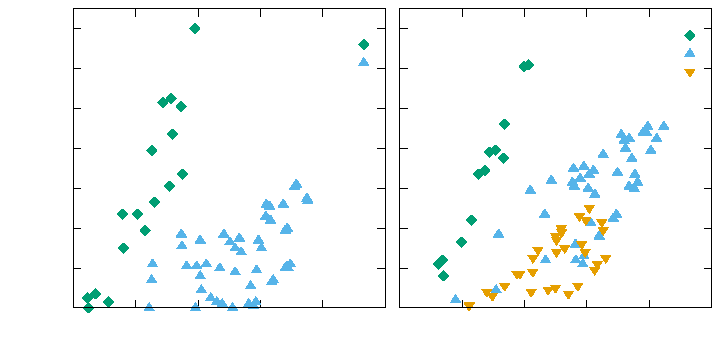
\includegraphics[width={325.00bp},height={127.00bp}]{Figs/DvsDBS}}%
    \gplfronttext
  \end{picture}%
\endgroup
 
    \caption[Q\textsubscript{0} and Q\textsubscript{1} DBS populations]{Q\textsubscript{0} and Q\textsubscript{1} DBS populations assigned to the DBS surfaces from Figures \ref{fig:Q0_maps} and \ref{fig:Q1_maps}.}
    \label{fig:D_vsDBS}
\end{figure}

\subsection{Interaction with small molecules}

Subsequent to the characterisation of the isolated quinones, the focus shifts to the interaction of their anionic states in the presence of small molecules. Recognising that chemical processes in nature do not occur in a vacuum and that environmental interactions are crucial, this work investigates these effects by considering small molecular clusters. Figure \ref{fig:scan_X} shows the interactions between Q\textsubscript{0} (region B, $\mathrm{\mu = 3.4~Debye}$, $\mathrm{EA_{DBS} = 6~meV}$), and selected molecules: methane ($\mathrm{\mu = 0~Debye}$), ammonia ($\mathrm{\mu = 1.47~Debye}$), water ($\mathrm{\mu = 1.85}$ Debye), and hydrogen fluoride ($\mathrm{\mu = 1.82~Debye}$). For these model systems, the dipole of the solvent molecule was oriented to interact either constructively or destructively with the quinone's dipole. In the case of methane, which has no dipole moment, it is shown in both cases for comparison. The intermolecular distance was systematically varied from 30 down to 4 \r{A}. The resulting effects on the VBS and DBS energies, are presented in Figure \ref{fig:scan_X}. It is important to note that none of these molecules support an anionic state on their own. The DBS of a representative Q\textsubscript{0} + water system for each of the two orientations is shown in Figure \ref{fig:Q1_dyson}.\\

\begin{figure}[th!]
    \centering
    \small
    % GNUPLOT: LaTeX picture with Postscript
\begingroup
  \makeatletter
  \providecommand\color[2][]{%
    \GenericError{(gnuplot) \space\space\space\@spaces}{%
      Package color not loaded in conjunction with
      terminal option `colourtext'%
    }{See the gnuplot documentation for explanation.%
    }{Either use 'blacktext' in gnuplot or load the package
      color.sty in LaTeX.}%
    \renewcommand\color[2][]{}%
  }%
  \providecommand\includegraphics[2][]{%
    \GenericError{(gnuplot) \space\space\space\@spaces}{%
      Package graphicx or graphics not loaded%
    }{See the gnuplot documentation for explanation.%
    }{The gnuplot epslatex terminal needs graphicx.sty or graphics.sty.}%
    \renewcommand\includegraphics[2][]{}%
  }%
  \providecommand\rotatebox[2]{#2}%
  \@ifundefined{ifGPcolor}{%
    \newif\ifGPcolor
    \GPcolortrue
  }{}%
  \@ifundefined{ifGPblacktext}{%
    \newif\ifGPblacktext
    \GPblacktexttrue
  }{}%
  % define a \g@addto@macro without @ in the name:
  \let\gplgaddtomacro\g@addto@macro
  % define empty templates for all commands taking text:
  \gdef\gplbacktext{}%
  \gdef\gplfronttext{}%
  \makeatother
  \ifGPblacktext
    % no textcolor at all
    \def\colorrgb#1{}%
    \def\colorgray#1{}%
  \else
    % gray or color?
    \ifGPcolor
      \def\colorrgb#1{\color[rgb]{#1}}%
      \def\colorgray#1{\color[gray]{#1}}%
      \expandafter\def\csname LTw\endcsname{\color{white}}%
      \expandafter\def\csname LTb\endcsname{\color{black}}%
      \expandafter\def\csname LTa\endcsname{\color{black}}%
      \expandafter\def\csname LT0\endcsname{\color[rgb]{1,0,0}}%
      \expandafter\def\csname LT1\endcsname{\color[rgb]{0,1,0}}%
      \expandafter\def\csname LT2\endcsname{\color[rgb]{0,0,1}}%
      \expandafter\def\csname LT3\endcsname{\color[rgb]{1,0,1}}%
      \expandafter\def\csname LT4\endcsname{\color[rgb]{0,1,1}}%
      \expandafter\def\csname LT5\endcsname{\color[rgb]{1,1,0}}%
      \expandafter\def\csname LT6\endcsname{\color[rgb]{0,0,0}}%
      \expandafter\def\csname LT7\endcsname{\color[rgb]{1,0.3,0}}%
      \expandafter\def\csname LT8\endcsname{\color[rgb]{0.5,0.5,0.5}}%
    \else
      % gray
      \def\colorrgb#1{\color{black}}%
      \def\colorgray#1{\color[gray]{#1}}%
      \expandafter\def\csname LTw\endcsname{\color{white}}%
      \expandafter\def\csname LTb\endcsname{\color{black}}%
      \expandafter\def\csname LTa\endcsname{\color{black}}%
      \expandafter\def\csname LT0\endcsname{\color{black}}%
      \expandafter\def\csname LT1\endcsname{\color{black}}%
      \expandafter\def\csname LT2\endcsname{\color{black}}%
      \expandafter\def\csname LT3\endcsname{\color{black}}%
      \expandafter\def\csname LT4\endcsname{\color{black}}%
      \expandafter\def\csname LT5\endcsname{\color{black}}%
      \expandafter\def\csname LT6\endcsname{\color{black}}%
      \expandafter\def\csname LT7\endcsname{\color{black}}%
      \expandafter\def\csname LT8\endcsname{\color{black}}%
    \fi
  \fi
    \setlength{\unitlength}{0.0500bp}%
    \ifx\gptboxheight\undefined%
      \newlength{\gptboxheight}%
      \newlength{\gptboxwidth}%
      \newsavebox{\gptboxtext}%
    \fi%
    \setlength{\fboxrule}{0.5pt}%
    \setlength{\fboxsep}{1pt}%
    \definecolor{tbcol}{rgb}{1,1,1}%
\begin{picture}(9060.00,9060.00)%
    \gplgaddtomacro\gplbacktext{%
      \csname LTb\endcsname%%
      \put(444,7172){\makebox(0,0)[r]{\strut{}-60}}%
      \csname LTb\endcsname%%
      \put(444,7603){\makebox(0,0)[r]{\strut{}-45}}%
      \csname LTb\endcsname%%
      \put(444,8034){\makebox(0,0)[r]{\strut{}-30}}%
      \csname LTb\endcsname%%
      \put(444,8465){\makebox(0,0)[r]{\strut{}-15}}%
      \csname LTb\endcsname%%
      \put(444,8896){\makebox(0,0)[r]{\strut{}0}}%
      \csname LTb\endcsname%%
      \put(1171,6852){\makebox(0,0){\strut{}}}%
      \csname LTb\endcsname%%
      \put(2745,6852){\makebox(0,0){\strut{}}}%
      \csname LTb\endcsname%%
      \put(4319,6852){\makebox(0,0){\strut{}}}%
      \csname LTb\endcsname%%
      \put(5892,6852){\makebox(0,0){\strut{}}}%
      \csname LTb\endcsname%%
      \put(7466,6852){\makebox(0,0){\strut{}}}%
      \csname LTb\endcsname%%
      \put(9039,6852){\makebox(0,0){\strut{}}}%
      \csname LTb\endcsname%%
      \put(4791,7229){\makebox(0,0){\strut{}DBS Opposing}}%
    }%
    \gplgaddtomacro\gplfronttext{%
    }%
    \gplgaddtomacro\gplbacktext{%
      \csname LTb\endcsname%%
      \put(444,4836){\makebox(0,0)[r]{\strut{}-2.6}}%
      \csname LTb\endcsname%%
      \put(444,5238){\makebox(0,0)[r]{\strut{}-2.4}}%
      \csname LTb\endcsname%%
      \put(444,5640){\makebox(0,0)[r]{\strut{}-2.2}}%
      \csname LTb\endcsname%%
      \put(444,6043){\makebox(0,0)[r]{\strut{}-2.0}}%
      \csname LTb\endcsname%%
      \put(444,6445){\makebox(0,0)[r]{\strut{}-1.8}}%
      \csname LTb\endcsname%%
      \put(444,6847){\makebox(0,0)[r]{\strut{}-1.6}}%
      \csname LTb\endcsname%%
      \put(1171,4660){\makebox(0,0){\strut{}}}%
      \csname LTb\endcsname%%
      \put(2745,4660){\makebox(0,0){\strut{}}}%
      \csname LTb\endcsname%%
      \put(4319,4660){\makebox(0,0){\strut{}}}%
      \csname LTb\endcsname%%
      \put(5892,4660){\makebox(0,0){\strut{}}}%
      \csname LTb\endcsname%%
      \put(7466,4660){\makebox(0,0){\strut{}}}%
      \csname LTb\endcsname%%
      \put(9039,4660){\makebox(0,0){\strut{}}}%
      \csname LTb\endcsname%%
      \put(4791,5037){\makebox(0,0){\strut{}VBS Opposing}}%
    }%
    \gplgaddtomacro\gplfronttext{%
    }%
    \gplgaddtomacro\gplbacktext{%
      \csname LTb\endcsname%%
      \put(444,2644){\makebox(0,0)[r]{\strut{}-80}}%
      \csname LTb\endcsname%%
      \put(444,3117){\makebox(0,0)[r]{\strut{}-60}}%
      \csname LTb\endcsname%%
      \put(444,3590){\makebox(0,0)[r]{\strut{}-40}}%
      \csname LTb\endcsname%%
      \put(444,4063){\makebox(0,0)[r]{\strut{}-20}}%
      \csname LTb\endcsname%%
      \put(444,4537){\makebox(0,0)[r]{\strut{}0}}%
      \csname LTb\endcsname%%
      \put(1171,2468){\makebox(0,0){\strut{}}}%
      \csname LTb\endcsname%%
      \put(2745,2468){\makebox(0,0){\strut{}}}%
      \csname LTb\endcsname%%
      \put(4319,2468){\makebox(0,0){\strut{}}}%
      \csname LTb\endcsname%%
      \put(5892,2468){\makebox(0,0){\strut{}}}%
      \csname LTb\endcsname%%
      \put(7466,2468){\makebox(0,0){\strut{}}}%
      \csname LTb\endcsname%%
      \put(9039,2468){\makebox(0,0){\strut{}}}%
      \csname LTb\endcsname%%
      \put(4791,2845){\makebox(0,0){\strut{}DBS Parallel}}%
    }%
    \gplgaddtomacro\gplfronttext{%
    }%
    \gplgaddtomacro\gplbacktext{%
      \csname LTb\endcsname%%
      \put(444,452){\makebox(0,0)[r]{\strut{}-2.0}}%
      \csname LTb\endcsname%%
      \put(444,1122){\makebox(0,0)[r]{\strut{}-1.8}}%
      \csname LTb\endcsname%%
      \put(444,1792){\makebox(0,0)[r]{\strut{}-1.6}}%
      \csname LTb\endcsname%%
      \put(444,2463){\makebox(0,0)[r]{\strut{}-1.4}}%
      \csname LTb\endcsname%%
      \put(1171,276){\makebox(0,0){\strut{}$5$}}%
      \csname LTb\endcsname%%
      \put(2745,276){\makebox(0,0){\strut{}$10$}}%
      \csname LTb\endcsname%%
      \put(4319,276){\makebox(0,0){\strut{}$15$}}%
      \csname LTb\endcsname%%
      \put(5892,276){\makebox(0,0){\strut{}$20$}}%
      \csname LTb\endcsname%%
      \put(7466,276){\makebox(0,0){\strut{}$25$}}%
      \csname LTb\endcsname%%
      \put(9039,276){\makebox(0,0){\strut{}$30$}}%
      \csname LTb\endcsname%%
      \put(4791,653){\makebox(0,0){\strut{}VBS Parallel}}%
    }%
    \gplgaddtomacro\gplfronttext{%
      \csname LTb\endcsname%%
      \put(4791,12){\makebox(0,0){\strut{}Distance (\AA)}}%
    }%
    \gplbacktext
    \put(0,0){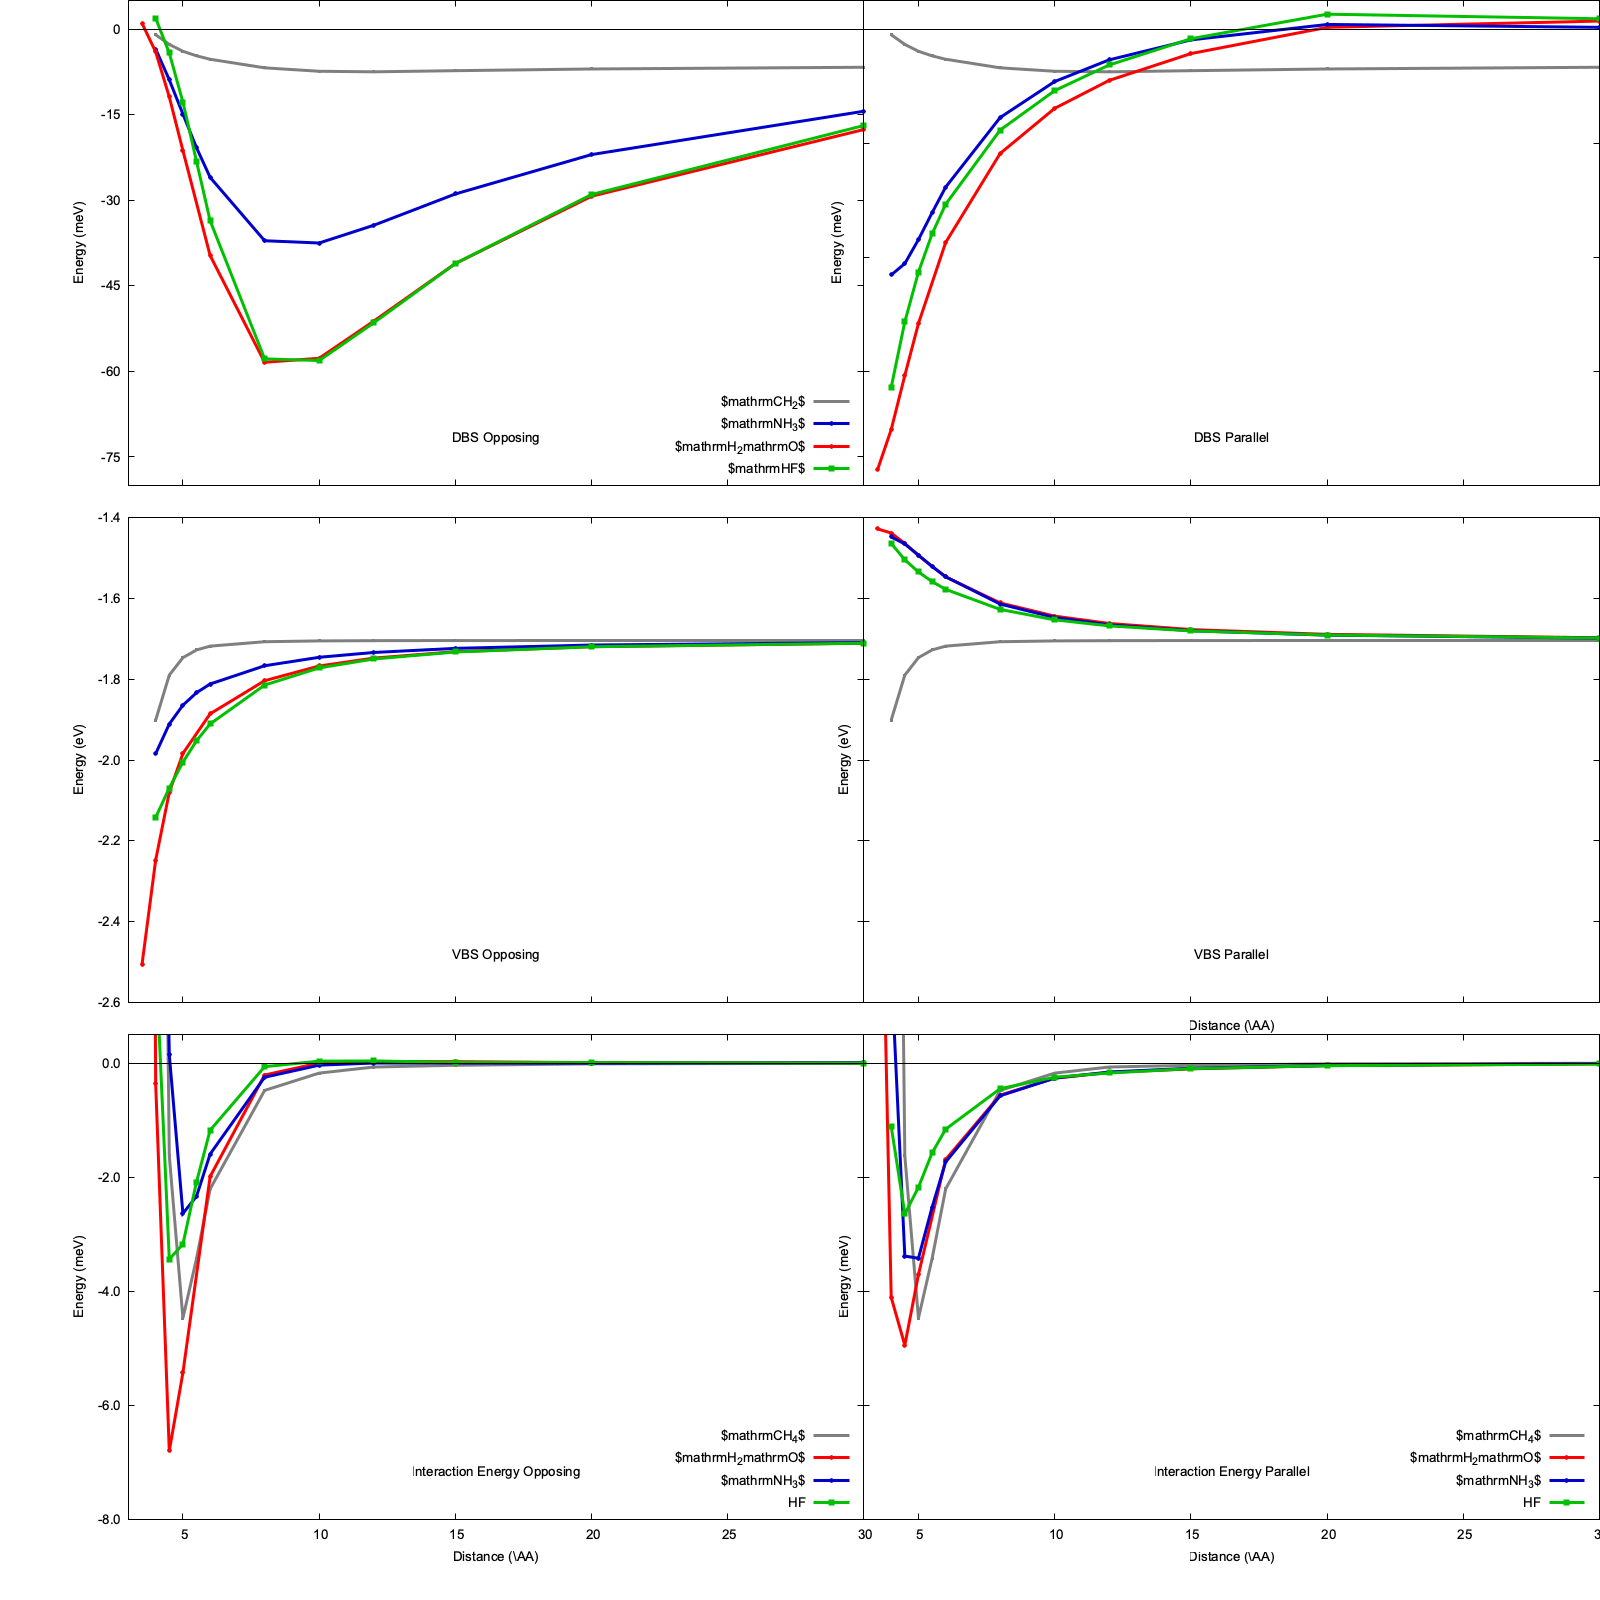
\includegraphics[width={453.00bp},height={453.00bp}]{chapters/results/image/scan_all}}%
    \gplfronttext
  \end{picture}%
\endgroup

    %% GNUPLOT: LaTeX picture with Postscript
\begingroup
  \makeatletter
  \providecommand\color[2][]{%
    \GenericError{(gnuplot) \space\space\space\@spaces}{%
      Package color not loaded in conjunction with
      terminal option `colourtext'%
    }{See the gnuplot documentation for explanation.%
    }{Either use 'blacktext' in gnuplot or load the package
      color.sty in LaTeX.}%
    \renewcommand\color[2][]{}%
  }%
  \providecommand\includegraphics[2][]{%
    \GenericError{(gnuplot) \space\space\space\@spaces}{%
      Package graphicx or graphics not loaded%
    }{See the gnuplot documentation for explanation.%
    }{The gnuplot epslatex terminal needs graphicx.sty or graphics.sty.}%
    \renewcommand\includegraphics[2][]{}%
  }%
  \providecommand\rotatebox[2]{#2}%
  \@ifundefined{ifGPcolor}{%
    \newif\ifGPcolor
    \GPcolortrue
  }{}%
  \@ifundefined{ifGPblacktext}{%
    \newif\ifGPblacktext
    \GPblacktexttrue
  }{}%
  % define a \g@addto@macro without @ in the name:
  \let\gplgaddtomacro\g@addto@macro
  % define empty templates for all commands taking text:
  \gdef\gplbacktext{}%
  \gdef\gplfronttext{}%
  \makeatother
  \ifGPblacktext
    % no textcolor at all
    \def\colorrgb#1{}%
    \def\colorgray#1{}%
  \else
    % gray or color?
    \ifGPcolor
      \def\colorrgb#1{\color[rgb]{#1}}%
      \def\colorgray#1{\color[gray]{#1}}%
      \expandafter\def\csname LTw\endcsname{\color{white}}%
      \expandafter\def\csname LTb\endcsname{\color{black}}%
      \expandafter\def\csname LTa\endcsname{\color{black}}%
      \expandafter\def\csname LT0\endcsname{\color[rgb]{1,0,0}}%
      \expandafter\def\csname LT1\endcsname{\color[rgb]{0,1,0}}%
      \expandafter\def\csname LT2\endcsname{\color[rgb]{0,0,1}}%
      \expandafter\def\csname LT3\endcsname{\color[rgb]{1,0,1}}%
      \expandafter\def\csname LT4\endcsname{\color[rgb]{0,1,1}}%
      \expandafter\def\csname LT5\endcsname{\color[rgb]{1,1,0}}%
      \expandafter\def\csname LT6\endcsname{\color[rgb]{0,0,0}}%
      \expandafter\def\csname LT7\endcsname{\color[rgb]{1,0.3,0}}%
      \expandafter\def\csname LT8\endcsname{\color[rgb]{0.5,0.5,0.5}}%
    \else
      % gray
      \def\colorrgb#1{\color{black}}%
      \def\colorgray#1{\color[gray]{#1}}%
      \expandafter\def\csname LTw\endcsname{\color{white}}%
      \expandafter\def\csname LTb\endcsname{\color{black}}%
      \expandafter\def\csname LTa\endcsname{\color{black}}%
      \expandafter\def\csname LT0\endcsname{\color{black}}%
      \expandafter\def\csname LT1\endcsname{\color{black}}%
      \expandafter\def\csname LT2\endcsname{\color{black}}%
      \expandafter\def\csname LT3\endcsname{\color{black}}%
      \expandafter\def\csname LT4\endcsname{\color{black}}%
      \expandafter\def\csname LT5\endcsname{\color{black}}%
      \expandafter\def\csname LT6\endcsname{\color{black}}%
      \expandafter\def\csname LT7\endcsname{\color{black}}%
      \expandafter\def\csname LT8\endcsname{\color{black}}%
    \fi
  \fi
    \setlength{\unitlength}{0.0500bp}%
    \ifx\gptboxheight\undefined%
      \newlength{\gptboxheight}%
      \newlength{\gptboxwidth}%
      \newsavebox{\gptboxtext}%
    \fi%
    \setlength{\fboxrule}{0.5pt}%
    \setlength{\fboxsep}{1pt}%
    \definecolor{tbcol}{rgb}{1,1,1}%
\begin{picture}(6980.00,3200.00)%
    \gplgaddtomacro\gplbacktext{%
      \csname LTb\endcsname%%
      \put(598,1728){\makebox(0,0)[r]{\strut{}-60}}%
      \csname LTb\endcsname%%
      \put(598,2048){\makebox(0,0)[r]{\strut{}-45}}%
      \csname LTb\endcsname%%
      \put(598,2369){\makebox(0,0)[r]{\strut{}-30}}%
      \csname LTb\endcsname%%
      \put(598,2689){\makebox(0,0)[r]{\strut{}-15}}%
      \csname LTb\endcsname%%
      \put(598,3009){\makebox(0,0)[r]{\strut{}0}}%
      \csname LTb\endcsname%%
      \put(1149,1445){\makebox(0,0){\strut{}}}%
      \csname LTb\endcsname%%
      \put(2283,1445){\makebox(0,0){\strut{}}}%
      \csname LTb\endcsname%%
      \put(3418,1445){\makebox(0,0){\strut{}}}%
      \csname LTb\endcsname%%
      \put(4552,1445){\makebox(0,0){\strut{}}}%
      \csname LTb\endcsname%%
      \put(5686,1445){\makebox(0,0){\strut{}}}%
      \csname LTb\endcsname%%
      \put(6820,1445){\makebox(0,0){\strut{}}}%
      \csname LTb\endcsname%%
      \put(3758,1771){\makebox(0,0){\strut{}DBS Opposing}}%
    }%
    \gplgaddtomacro\gplfronttext{%
      \csname LTb\endcsname%%
      \put(45,2369){\rotatebox{-270.00}{\makebox(0,0){\strut{}Energy (meV)}}}%
    }%
    \gplgaddtomacro\gplbacktext{%
      \csname LTb\endcsname%%
      \put(598,31){\makebox(0,0)[r]{\strut{}-2.6}}%
      \csname LTb\endcsname%%
      \put(598,330){\makebox(0,0)[r]{\strut{}-2.4}}%
      \csname LTb\endcsname%%
      \put(598,629){\makebox(0,0)[r]{\strut{}-2.2}}%
      \csname LTb\endcsname%%
      \put(598,928){\makebox(0,0)[r]{\strut{}-2.0}}%
      \csname LTb\endcsname%%
      \put(598,1227){\makebox(0,0)[r]{\strut{}-1.8}}%
      \csname LTb\endcsname%%
      \put(598,1526){\makebox(0,0)[r]{\strut{}-1.6}}%
      \csname LTb\endcsname%%
      \put(3758,181){\makebox(0,0){\strut{}VBS Opposing}}%
    }%
    \gplgaddtomacro\gplfronttext{%
      \csname LTb\endcsname%%
      \put(45,779){\rotatebox{-270.00}{\makebox(0,0){\strut{}Energy (eV)}}}%
    }%
    \gplbacktext
    \put(0,0){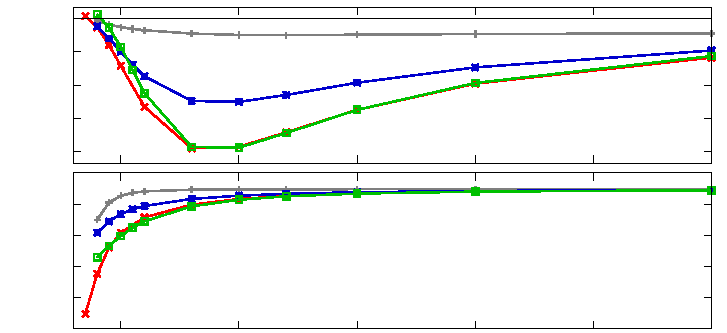
\includegraphics[width={349.00bp},height={160.00bp}]{scan_H}}%
    \gplfronttext
  \end{picture}%
\endgroup

    %% GNUPLOT: LaTeX picture with Postscript
\begingroup
  \makeatletter
  \providecommand\color[2][]{%
    \GenericError{(gnuplot) \space\space\space\@spaces}{%
      Package color not loaded in conjunction with
      terminal option `colourtext'%
    }{See the gnuplot documentation for explanation.%
    }{Either use 'blacktext' in gnuplot or load the package
      color.sty in LaTeX.}%
    \renewcommand\color[2][]{}%
  }%
  \providecommand\includegraphics[2][]{%
    \GenericError{(gnuplot) \space\space\space\@spaces}{%
      Package graphicx or graphics not loaded%
    }{See the gnuplot documentation for explanation.%
    }{The gnuplot epslatex terminal needs graphicx.sty or graphics.sty.}%
    \renewcommand\includegraphics[2][]{}%
  }%
  \providecommand\rotatebox[2]{#2}%
  \@ifundefined{ifGPcolor}{%
    \newif\ifGPcolor
    \GPcolortrue
  }{}%
  \@ifundefined{ifGPblacktext}{%
    \newif\ifGPblacktext
    \GPblacktexttrue
  }{}%
  % define a \g@addto@macro without @ in the name:
  \let\gplgaddtomacro\g@addto@macro
  % define empty templates for all commands taking text:
  \gdef\gplbacktext{}%
  \gdef\gplfronttext{}%
  \makeatother
  \ifGPblacktext
    % no textcolor at all
    \def\colorrgb#1{}%
    \def\colorgray#1{}%
  \else
    % gray or color?
    \ifGPcolor
      \def\colorrgb#1{\color[rgb]{#1}}%
      \def\colorgray#1{\color[gray]{#1}}%
      \expandafter\def\csname LTw\endcsname{\color{white}}%
      \expandafter\def\csname LTb\endcsname{\color{black}}%
      \expandafter\def\csname LTa\endcsname{\color{black}}%
      \expandafter\def\csname LT0\endcsname{\color[rgb]{1,0,0}}%
      \expandafter\def\csname LT1\endcsname{\color[rgb]{0,1,0}}%
      \expandafter\def\csname LT2\endcsname{\color[rgb]{0,0,1}}%
      \expandafter\def\csname LT3\endcsname{\color[rgb]{1,0,1}}%
      \expandafter\def\csname LT4\endcsname{\color[rgb]{0,1,1}}%
      \expandafter\def\csname LT5\endcsname{\color[rgb]{1,1,0}}%
      \expandafter\def\csname LT6\endcsname{\color[rgb]{0,0,0}}%
      \expandafter\def\csname LT7\endcsname{\color[rgb]{1,0.3,0}}%
      \expandafter\def\csname LT8\endcsname{\color[rgb]{0.5,0.5,0.5}}%
    \else
      % gray
      \def\colorrgb#1{\color{black}}%
      \def\colorgray#1{\color[gray]{#1}}%
      \expandafter\def\csname LTw\endcsname{\color{white}}%
      \expandafter\def\csname LTb\endcsname{\color{black}}%
      \expandafter\def\csname LTa\endcsname{\color{black}}%
      \expandafter\def\csname LT0\endcsname{\color{black}}%
      \expandafter\def\csname LT1\endcsname{\color{black}}%
      \expandafter\def\csname LT2\endcsname{\color{black}}%
      \expandafter\def\csname LT3\endcsname{\color{black}}%
      \expandafter\def\csname LT4\endcsname{\color{black}}%
      \expandafter\def\csname LT5\endcsname{\color{black}}%
      \expandafter\def\csname LT6\endcsname{\color{black}}%
      \expandafter\def\csname LT7\endcsname{\color{black}}%
      \expandafter\def\csname LT8\endcsname{\color{black}}%
    \fi
  \fi
    \setlength{\unitlength}{0.0500bp}%
    \ifx\gptboxheight\undefined%
      \newlength{\gptboxheight}%
      \newlength{\gptboxwidth}%
      \newsavebox{\gptboxtext}%
    \fi%
    \setlength{\fboxrule}{0.5pt}%
    \setlength{\fboxsep}{1pt}%
    \definecolor{tbcol}{rgb}{1,1,1}%
\begin{picture}(6980.00,3480.00)%
    \gplgaddtomacro\gplbacktext{%
      \csname LTb\endcsname%%
      \put(598,2006){\makebox(0,0)[r]{\strut{}-80}}%
      \csname LTb\endcsname%%
      \put(598,2332){\makebox(0,0)[r]{\strut{}-60}}%
      \csname LTb\endcsname%%
      \put(598,2658){\makebox(0,0)[r]{\strut{}-40}}%
      \csname LTb\endcsname%%
      \put(598,2983){\makebox(0,0)[r]{\strut{}-20}}%
      \csname LTb\endcsname%%
      \put(598,3309){\makebox(0,0)[r]{\strut{}0}}%
      \csname LTb\endcsname%%
      \put(1149,1830){\makebox(0,0){\strut{}}}%
      \csname LTb\endcsname%%
      \put(2283,1830){\makebox(0,0){\strut{}}}%
      \csname LTb\endcsname%%
      \put(3418,1830){\makebox(0,0){\strut{}}}%
      \csname LTb\endcsname%%
      \put(4552,1830){\makebox(0,0){\strut{}}}%
      \csname LTb\endcsname%%
      \put(5686,1830){\makebox(0,0){\strut{}}}%
      \csname LTb\endcsname%%
      \put(6820,1830){\makebox(0,0){\strut{}}}%
      \csname LTb\endcsname%%
      \put(3758,2145){\makebox(0,0){\strut{}DBS Parallel}}%
    }%
    \gplgaddtomacro\gplfronttext{%
      \csname LTb\endcsname%%
      \put(45,2698){\rotatebox{-270.00}{\makebox(0,0){\strut{}Energy (meV)}}}%
    }%
    \gplgaddtomacro\gplbacktext{%
      \csname LTb\endcsname%%
      \put(598,519){\makebox(0,0)[r]{\strut{}-2.0}}%
      \csname LTb\endcsname%%
      \put(598,980){\makebox(0,0)[r]{\strut{}-1.8}}%
      \csname LTb\endcsname%%
      \put(598,1441){\makebox(0,0)[r]{\strut{}-1.6}}%
      \csname LTb\endcsname%%
      \put(598,1902){\makebox(0,0)[r]{\strut{}-1.4}}%
      \csname LTb\endcsname%%
      \put(1149,343){\makebox(0,0){\strut{}$5$}}%
      \csname LTb\endcsname%%
      \put(2283,343){\makebox(0,0){\strut{}$10$}}%
      \csname LTb\endcsname%%
      \put(3418,343){\makebox(0,0){\strut{}$15$}}%
      \csname LTb\endcsname%%
      \put(4552,343){\makebox(0,0){\strut{}$20$}}%
      \csname LTb\endcsname%%
      \put(5686,343){\makebox(0,0){\strut{}$25$}}%
      \csname LTb\endcsname%%
      \put(6820,343){\makebox(0,0){\strut{}$30$}}%
      \csname LTb\endcsname%%
      \put(3758,657){\makebox(0,0){\strut{}VBS Parallel}}%
    }%
    \gplgaddtomacro\gplfronttext{%
      \csname LTb\endcsname%%
      \put(45,1210){\rotatebox{-270.00}{\makebox(0,0){\strut{}Energy (eV)}}}%
      \csname LTb\endcsname%%
      \put(3758,79){\makebox(0,0){\strut{}Distance (\AA)}}%
    }%
    \gplbacktext
    \put(0,0){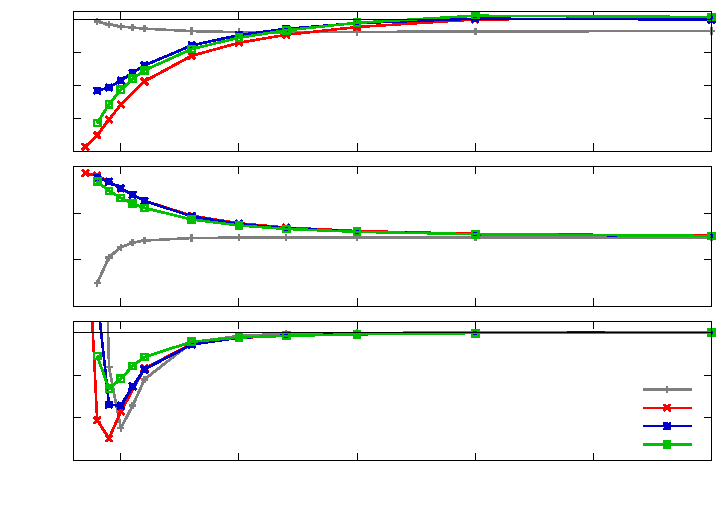
\includegraphics[width={349.00bp},height={174.00bp}]{scan_X}}%
    \gplfronttext
  \end{picture}%
\endgroup

    %figsize is set in image/test.gp 
    \caption[Q\textsubscript{0} interaction with small molecules]{Q\textsubscript{0} interaction with small molecules. From top to bottom: DBS with opposing dipoles, VBS with opposing dipoles, DBS with aligned dipoles, and VBS with aligned dipoles.}
    \label{fig:scan_X}
\end{figure}

Considering the DBS, when the solvent and quinone dipoles are opposed, polar molecules induce a wide well with a minimum at around 8 \r{A}. The electron binding energy of the DBS reaches 60 meV with both water and HF, and 37 meV with ammonia. This represents a more than tenfold increase compared to the 5.4 meV binding energy of the isolated quinone. Stabilisation by methane is considerably weaker, as it arises solely from dispersion forces. The similarity between the water and HF interaction curves is noteworthy; they overlap almost perfectly across most of the separation range. This congruence is attributed to their comparable dipole moments (1.85 D for water; 1.82 D for HF). At large separations, the specific electronic structures of these solvent molecules are less influential, and the DBS primarily experiences the effect of their dipole moments. The interaction with ammonia is weaker due to its smaller dipole moment of 1.47 D. This scenario is characteristic of a solvated electron within a `cavity' \cite{jordan2003theory,herbert2019structure}. At an intermolecular distance of approximately 4 \r{A}, the interaction becomes repulsive for all molecules studied due to steric interactions, causing the DBS to become unbound due to steric hindrance.\\

Conversely, with parallel dipole orientations, polar molecules exhibit repulsion at large distances. This is attributable to the negative end of the solvent dipole destabilising the DBS. At shorter ranges, however, the local dipoles combine constructively, thereby stabilising the binding energy. For water, which possesses the largest dipole moment, the DBS attains an electron binding energy of 80 meV, with the total system dipole moment being 6.1 Debye. Such configurations have recently been observed in photoelectron spectroscopy experiments \cite{clarke2025role} and are thought to play an important role in the transfer of a VBS to a solvated electron.\\

\begin{figure}[h]
  \centering
    \begin{minipage}[b]{0.3\textwidth}
    \centering
      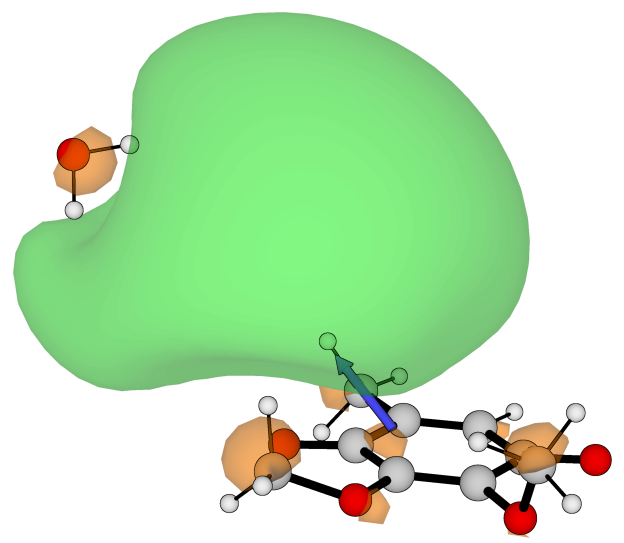
\includegraphics[width=0.9\textwidth]{chapters/results/image/Q0_H2O_H.png}
      %\small\emph{Region A \\$(0,0)~\mu=2.6~D$ E=12.2~meV}
  \end{minipage}
  \hfill
  \begin{minipage}[b]{0.3\textwidth}
    \centering
    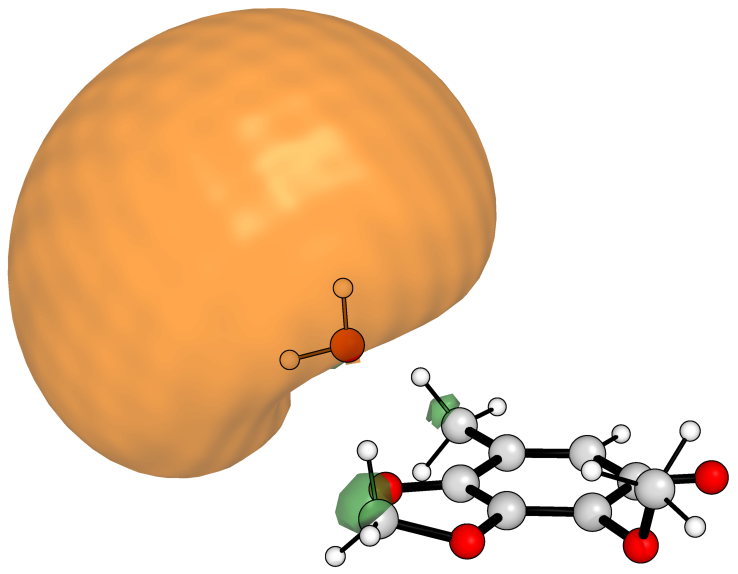
\includegraphics[width=1\textwidth]{chapters/results/image/Q0_H2O_O.png}
    %\small\emph{Region C \\$(-60,160)~\mu=2.9~D$, $E=5.0~meV$}
  \end{minipage}
  \hfill
  \begin{minipage}[b]{0.3\textwidth}
    \centering
    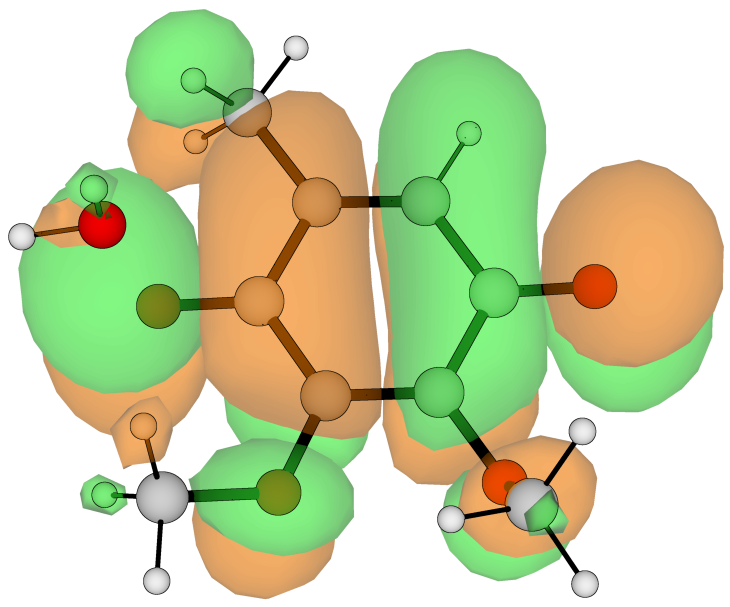
\includegraphics[width=0.9\textwidth]{chapters/results/image/Q0_H2O_VBS.png}
    %\small\emph{Region C \\$(-60,160)~\mu=2.9~D$, $E=5.0~meV$}
  \end{minipage}
  \caption[Dyson orbitals of Q0+water]{Dyson orbitals of Q0 + water calculated with RI-EA-EOM-CC2/aug-cc-pVDZ+6s3p. Left, system where the dipoles are pointing in opposite directions at an intermolecular distance of 8 \r{A}. Middle: dipoles aligned at an intermolecular distance of 4 \r{A}. Right: VBS of Q0 and a water molecule at 4 \r{A}. The isosurface is set to 0.01 a.u. and the dipole moment vector is shown as a blue arrow with origin at the centre of mass.}
  \label{fig:Q0_H2O_dyson}
\end{figure}

The interaction also significantly affects the VBS. When the dipoles are opposed, \textit{i.e.}, the positive end of the solvent dipole is oriented towards the excess electronic charge of the quinone, the VBS is strongly stabilised at short intermolecular distances. With water, the VBS achieves a VEA of 2.5 eV, an increase of over 0.8 eV compared to the isolated quinone. A similar effect is observed for HF, yielding a VEA of 2.5 eV, while the stabilisation is less pronounced for ammonia and methane. A comparison of the influence of surrounding molecules on the VBS with that of methoxy chain rotation, as discussed in section \ref{sec:Q0_maps}, reveals that intermolecular interactions can be considerably more influential. The protein environment has probably a larger effect on the CoQ EA than the orientation adopted by the methoxy chains.\\

If the dipoles are aligned, the negative end of the solvent dipole interacts with the VBS and is destabilised. A similar and unfavourable trend is observed for the three polar molecules. At an intermolecular distance of 4 \r{A}, the VEA decreases to approximately 1.4 eV. The destabilisation arises from the negative end of the solvent dipole repelling the excess electron density of the quinone.\\

Regarding the total interaction energy of the neutral system, it is important to note that the interaction with the solvent molecules is always attractive. Additionally the dipole-dipole interaction is not the main driver of the energy curve, as it can be observed how for the case of water of HF, opposing dipoles lead to a deeper well than aligned dipoles. This observation can be rationalised by a similar argument to that of the VBS, which is a \textpi \textsuperscript{*} state. The interactions of the dipole of the solvent molecule with the \textpi system of the quinone is stronger than that of the dipole-dipole energy.
%\subsection{Effect of Nearby Amionacids}


%%%%%%%%%%%%%%%%%%%%%%%%%%%%%%%%%%%%%%%%%%%%%%%%%%
% Keep the following \cleardoublepage at the end of this file, 
% otherwise \includeonly includes empty pages.
\cleardoublepage

% vim: tw=70 nocindent expandtab foldmethod=marker foldmarker={{{}{,}{}}}